\clearpage
\phantomsection
\section*{五、CEC 下的业务感知 Batching 参数优化方法}
\addcontentsline{toc}{section}{五、CEC 下的业务感知 Batching 参数优化方法}

LLM serving 中的 batching 不再只是传统 DNN 推理里的固定 batch size 选择。一次 LLM 请求通常先经历 prefill，再进入逐 token decode；请求到达时间、prompt 长度、输出长度、SLO、KV Cache 占用和上下文复用机会都会随时间变化。因此，batching 的核心问题可以定义为：在给定请求队列、实例负载、KV 状态和协作节点间链路条件下，动态决定哪些请求进入 batch、batch 在什么粒度更新、prefill 与 decode 是否混合、长 prompt 是否切块、不同阶段是否解耦，从而在 TTFT、ITL、TPOT、E2E latency、throughput、goodput 和资源利用率之间取得平衡。Orca 将生成式 Transformer serving 的调度粒度推进到 iteration level \cite{yu2022orca}；vLLM 通过 PagedAttention 为 continuous batching 提供了 KV 内存管理基础 \cite{kwon2023efficient}；Sarathi-Serve 代表 chunked prefill 路线 \cite{agrawal2024taming}，DistServe 则代表 prefill/decode disaggregation 路线 \cite{zhong2024distserve}。
在 CEC 场景中，这个问题进一步复杂化。单个请求入口附近的节点或服务实例通常只有较小的请求池，单纯等待大 batch 会破坏 TTFT；边缘 GPU/NPU 显存有限，KV Cache 会限制可并发 decode 请求数；终端接入链路和边缘节点间链路状态会影响 prefill offloading、decode placement 和状态传输收益；不同业务还可能具有差异化 SLO，例如机器人控制、车联网辅助决策、工业现场问答和普通对话服务的最大等待时间并不相同。基于这些特点，本章以 batching 机制及 batch 更新粒度为分类主线，并将 SLO、KV Cache、多租户和推测验证等因素作为贯穿各类方法的调度约束。
这些横向因素分别影响请求接纳、batch 组成、KV 管理和执行顺序。例如，SOLA/JITServe 根据 SLO 约束控制请求接纳，vLLM 为 KV-aware continuous batching 提供内存管理基础，S-LoRA/Punica 中的多租户 adapter serving 会改变 batch 的组成方式和执行算子，AdaServe 和 MuxServe 则分别引入推测验证与多模型时空复用条件下的批处理决策。
本文将 CEC 下的业务感知 batching 参数优化划分为四类：
\begin{enumerate}
\item \textbf{Queue-level Dynamic / Admission Batching}：batch 在请求进入执行前根据到达情况、等待窗口、优先级、距离 deadline 的剩余时间或 admission threshold 动态组成。
\item \textbf{Continuous Batching / Iteration-level Batching}：以 decode iteration 或 token iteration 为边界动态维护 active batch，使完成请求退出、新请求或被抢占请求加入。
\item \textbf{Chunked Prefill / Blended Batching}：把长 prefill 切成 chunk，并与 decode token 或其他请求混合执行，缓解长 prompt 对 decode 的阻塞。
\item \textbf{Disaggregated Prefill-Decode Batching}：将 prefill 和 decode 分配给不同实例、资源池或协作节点，分别形成阶段 batch，并通过 KV/state transfer 衔接。
\end{enumerate}

这四类方法从 batch 的形成与更新粒度描述不同的批处理组织方式，彼此之间可以组合使用。本文以固定参数、按到达顺序形成批次的 Static-FIFO 作为实验基线；四类主体方法则分别面向请求接纳与动态组批、迭代级 active batch、prefill chunk 混合和 prefill/decode 阶段解耦。Queue-level dynamic/admission batching 可以引入 SLO-aware priority；Continuous batching 可以结合抢占、KV-aware admission 和 active set 调整，Orca~\cite{yu2022orca} 和 FastServe~\cite{wu2026fastserve} 分别体现了 iteration-level scheduling 与 preemptive scheduling 的代表路线；Chunked Prefill / Blended Batching 通常建立在 continuous batching runtime 之上，Sarathi-Serve~\cite{agrawal2024taming} 是这一方向的典型系统；Disaggregated Prefill-Decode Batching 则将两个阶段的 batch 分配到不同资源池，DistServe~\cite{zhong2024distserve} 是阶段解耦路线的代表。

表~\ref{tab:cec-batching-overview} 汇总了与 batching 执行机制直接相关的代表工作以及会改变批处理决策的横向机制；图~\ref{fig:cec-batching-taxonomy} 给出了四类方法在批次形成粒度上的分类主线。SLO-aware、multi-tenant、KV-aware、speculative verification、multi-model serving 和 inference/finetuning co-serving 贯穿上述分类，并通过请求优先级、batch 组成、显存占用和资源竞争影响调度结果。LoRA serving、多模型 serving 和 inference/finetuning co-serving 的关键问题在于，如何组织不同 adapter、模型或任务类型共享 batch 与 GPU 时间片，并在 SLO、显存和阶段干扰约束下确定执行顺序，因此也被纳入比较。

\begingroup
\scriptsize
\setlength{\tabcolsep}{1.4pt}
\renewcommand{\arraystretch}{1.35}
\emergencystretch=2em
\begin{longtable}{@{}>{\raggedright\arraybackslash\hspace{0pt}}p{0.035\textwidth} >{\raggedright\arraybackslash\hspace{0pt}}p{0.175\textwidth} >{\raggedright\arraybackslash\hspace{0pt}}p{0.095\textwidth} >{\raggedright\arraybackslash\hspace{0pt}}p{0.170\textwidth} >{\raggedright\arraybackslash\hspace{0pt}}p{0.155\textwidth} >{\raggedright\arraybackslash\hspace{0pt}}p{0.330\textwidth}@{}}
\caption{\textbf{CEC 下业务感知 Batching 参数优化方法相关工作}}
\label{tab:cec-batching-overview}\\
\toprule
\textbf{序号} & \textbf{代表工作} & \textbf{发表在哪} & \textbf{主归属} & \textbf{相关机制} & \textbf{方法关键词} \\
\midrule
1 & JITServe \cite{zhang2026jitserve} & NSDI 2026 & Queue-level Dynamic / Admission Batching & SLO-aware request admission & 根据请求 SLO deadline、剩余时间预算和当前服务带宽动态决定接纳、排序和组批 \\
\tabrowrule
2 & SOLA \cite{hong2025sola} & MLSys 2025 & Queue-level Dynamic / Admission Batching & SLO-aware scheduling；phase-aware scheduling & 根据成本模型预测 TTFT/TPOT 相对 SLO 的紧迫程度，对等待请求排序并决定谁优先进入 batch \\
\tabrowrule
3 & QLM \cite{jhaone} & AIOps@\newline ASPLOS 2024 & Queue-level Dynamic / Admission Batching & Queue management & 以满足端到端延迟 SLO 为目标，通过队列控制减少 head-of-line blocking 并提高 SLO attainment \\
\tabrowrule
4 & TimelyLLM \cite{ling2024timelyllm} & MobiSys 2026 & Queue-level Dynamic / Admission Batching & time utility；iteration-level control & 面向时间敏感应用，将 deadline 和 time utility 纳入 batch 接纳与请求优先级 \\
\tabrowrule
5 & Preble \cite{srivatsa2025preble} & ICLR 2025 & Queue-level Dynamic / Admission Batching & KV-aware admission；distributed prompt scheduling & 在分布式 serving 中把 prefix/KV cache 命中和负载均衡共同纳入请求分配，使共享 prompt 请求更容易进入可复用状态的实例 \\
\tabrowrule
6 & Fairness in Serving Large Language Models \cite{sheng2024fairness} & OSDI 2024 & Queue-level Dynamic / Admission Batching；Continuous / Iteration-level Batching & multi-tenant fairness；VTC & 在 continuous batching 机制上引入 Virtual Token Counter，用已服务 token 成本调整调度顺序，减少租户之间的服务不公平 \\
\tabrowrule
7 & Orca \cite{yu2022orca} & OSDI 2022 & Continuous / Iteration-level Batching & selective batching & 提出 iteration-level scheduling，新请求在 decode iteration 边界加入，完成请求及时退出 active batch \\
\tabrowrule
8 & FastServe \cite{wu2026fastserve} & NSDI 2026 & Continuous / Iteration-level Batching & preemptive scheduling & 在 continuous batching 基础上引入迭代级抢占，缓解长请求占用和尾延迟问题 \\
\tabrowrule
9 & TokenFlow \cite{chen2026tokenflow} & EuroSys 2026 & Continuous / Iteration-level Batching & streaming token scheduling & 以 token stream / scheduling interval 为控制粒度，动态做 admission、preemption 和 resumption \\
\tabrowrule
10 & vLLM \cite{kwon2023efficient} & SOSP 2023 & Continuous / Iteration-level Batching & KV block memory management & PagedAttention 用逻辑/物理 KV block 映射降低显存碎片，为更大的 active batch 提供内存基础 \\
\tabrowrule
11 & SGLang \cite{zheng2024sglang} & NeurIPS 2024 & Continuous / Iteration-level Batching & RadixAttention；prefix reuse & 通过 RadixAttention 自动匹配和复用共享前缀 KV，使复杂多轮、RAG 和 agent workload 的 active batch 更少重复 prefill \\
\tabrowrule
12 & Llumnix \cite{sun2024llumnix} & OSDI 2024 & Continuous / Iteration-level Batching & runtime rescheduling；live migration & 在多个 vLLM 实例之间迁移运行中请求及其内存状态，缓解 active batch 负载不均、优先级变化和尾延迟问题 \\
\tabrowrule
13 & Punica \cite{chen2024punica} & MLSys 2024 & Continuous / Iteration-level Batching & multi-tenant LoRA batching & 用 SGMV 等算子支持不同 LoRA adapter 请求共享同一基础模型 batch，降低多租户 LoRA serving 的显存和计算浪费 \\
\tabrowrule
14 & S-LoRA \cite{sheng2024slora} & MLSys 2024 & Continuous / Iteration-level Batching & heterogeneous adapter batching；unified paging & 通过统一分页管理 adapter 权重和 KV cache，并用定制 LoRA 算子支持大量 adapter 请求在同一 serving 实例中批处理 \\
\tabrowrule
15 & NanoFlow \cite{zhu2025nanoflow} & OSDI 2025 & Continuous / Iteration-level Batching；Chunked Prefill / Blended Batching & nano-batch scheduling & 将执行拆成 nano-batches 并搜索数量、大小和顺序，同时对长 prefill 做 token 粒度分块 \\
\tabrowrule
16 & Sarathi-Serve \cite{agrawal2024taming} & OSDI 2024 & Chunked Prefill / Blended Batching & chunked prefill；decode interleaving & 将长 prefill 切成 chunk，并与 decode 混合交错执行，平滑两阶段负载 \\
\tabrowrule
17 & Libra \cite{ruan2026libra} & NSDI 2026 & Chunked Prefill / Blended Batching & phase quota control & 在混合批次中调控 prefill 与 decode token 配额比例，降低两阶段算子干扰 \\
\tabrowrule
18 & A Hybrid Online and Offline Requests Inference Serving System for LLM in Private Computer Environment \cite{shen2025hybrid} & IEEE TC 2026 & Chunked Prefill / Blended Batching & online/offline mixed batching & 在同一 continuous batch 内组织在线 prefill/decode 与离线任务，在线优先、离线填充空闲资源 \\
\tabrowrule
19 & LLMStation \cite{he2025resource} & USENIX ATC 2025 & Chunked Prefill / Blended Batching & iteration-level multitasking；inference/tuning co-serving & 将 fine-tuning 任务改造成可挂起流水线，并在 iteration 粒度批处理 inference 与 tuning 请求，以提高 GPU 利用率同时满足 serving SLO \\
\tabrowrule
20 & FlexLLM \cite{oliaro2026flexllm} & NSDI 2026 & Chunked Prefill / Blended Batching & token-level co-serving；SLO-aware scheduling & 将 inference 和 PEFT finetuning 融合到 token 级执行，并优先保护 latency-sensitive inference 的 SLO，再利用空闲 token 预算推进 finetuning \\
\tabrowrule
21 & AdaServe \cite{li2026adaserve} & EuroSys 2026 & 横向机制：Speculative Verification Batching & multi-SLO speculative decoding & 按请求 SLO 定制 speculation tree，并通过 speculate-select-verify pipeline 形成验证批处理；它主要补充 multi-SLO 场景下的验证调度，而不是 prefill chunking \\
\tabrowrule
22 & DistServe \cite{zhong2024distserve} & OSDI 2024 & Disaggregated Prefill-Decode Batching & phase-specific workers & 将 compute-heavy prefill 与 memory/latency-sensitive decode 解耦到不同 worker pool \\
\tabrowrule
23 & Splitwise \cite{patel2024splitwise} & ISCA 2024 & Disaggregated Prefill-Decode Batching & prompt pool；token pool & 将 prompt computation 和 token generation 放到不同机器池，并分别匹配硬件资源 \\
\tabrowrule
24 & Mooncake \cite{qin2025mooncake} & USENIX FAST 2025 & Disaggregated Prefill-Decode Batching & distributed KV cache；global scheduling & 在 prefill/decode 解耦基础上构建分布式 KVCache，并按 KV 本地性和 SLO 调度实例 \\
\tabrowrule
25 & MuxServe \cite{duan2024muxserve} & ICML 2024 & 横向机制：Multi-model Multiplexed Batching & adaptive batch scheduling；spatial-temporal multiplexing & 面向多 LLM serving 联合做空间共置和时间复用，并利用 prefill/decode 阶段特征设计 adaptive batch scheduling，以提升多模型场景下的 SLO 吞吐 \\
\bottomrule
\end{longtable}
\endgroup

\begin{figure}[!htbp]
\centering
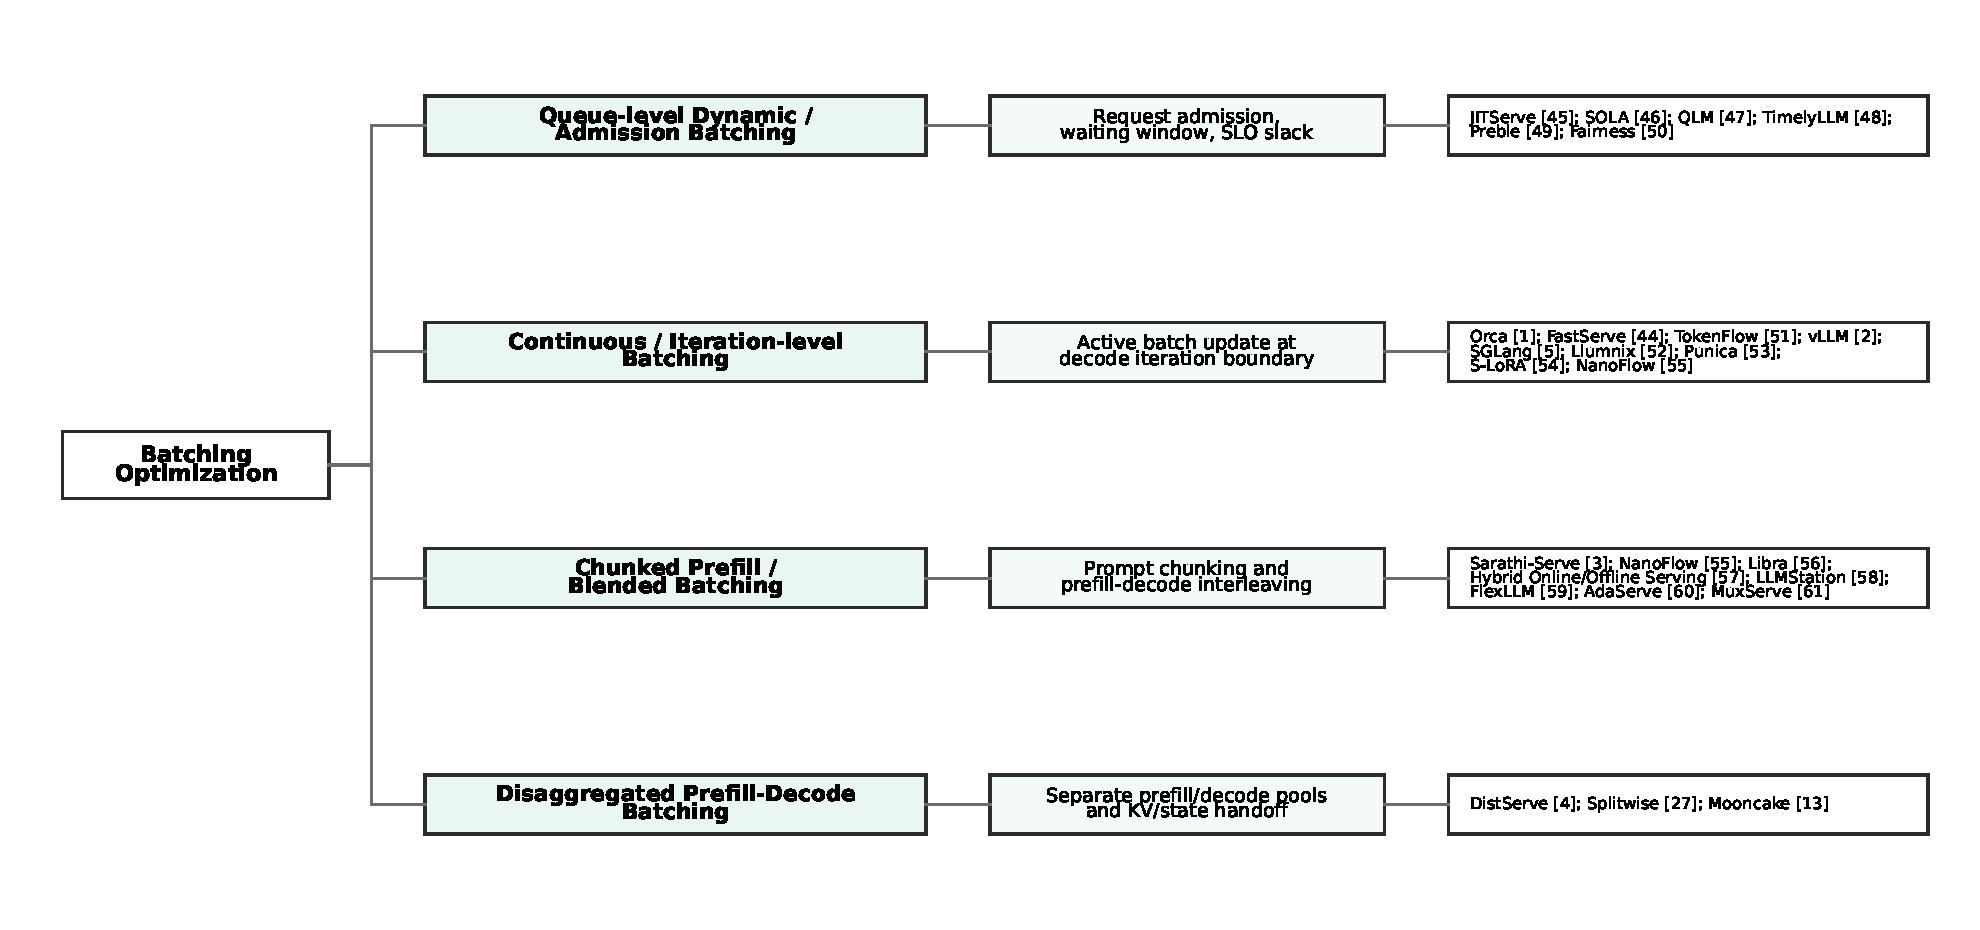
\includegraphics[width=\textwidth]{figures/ch5_batching_taxonomy.pdf}
\caption{\textbf{CEC 下业务感知 Batching 参数优化方法的分类树}}
\label{fig:cec-batching-taxonomy}
\end{figure}

\phantomsection
\subsection*{5.1 Queue-level Dynamic / Admission Batching}
\addcontentsline{toc}{subsection}{5.1 Queue-level Dynamic / Admission Batching}
Queue-level Dynamic / Admission Batching 要解决的是“固定等待固定 batch size 过于僵硬”的问题。真实 LLM 服务中，请求到达是随机的，prompt 长度、输出长度和 SLO 也不一致。如果系统仍按固定 batch size 或固定时间窗口组批，低负载时会等待过久，高负载时又可能把紧急请求排在队尾。因此，这类方法在请求进入执行前动态决定 batching window、batch membership、admission threshold 和请求优先级。JITServe 从 SLO-aware serving 角度建模请求服务带宽 \cite{zhang2026jitserve}，SOLA 以 state-aware scheduling 提高 SLO attainment \cite{hong2025sola}，QLM 关注队列管理和 head-of-line blocking \cite{jhaone}，TimelyLLM 则面向时间敏感机器人应用组织请求调度 \cite{ling2024timelyllm}。Preble 说明 prefix/KV locality 会改变请求分配 \cite{srivatsa2025preble}；Fairness in Serving Large Language Models 则说明多租户公平性也会改变请求排序和 token 服务顺序 \cite{sheng2024fairness}。

这种队列级决策可以抽象成图~\ref{fig:ch5-dynamic-admission-batching} 中的闭环：请求先等待，控制器再根据剩余时间预算决定立即执行还是继续合批。
\begin{figure}[!htbp]
\centering
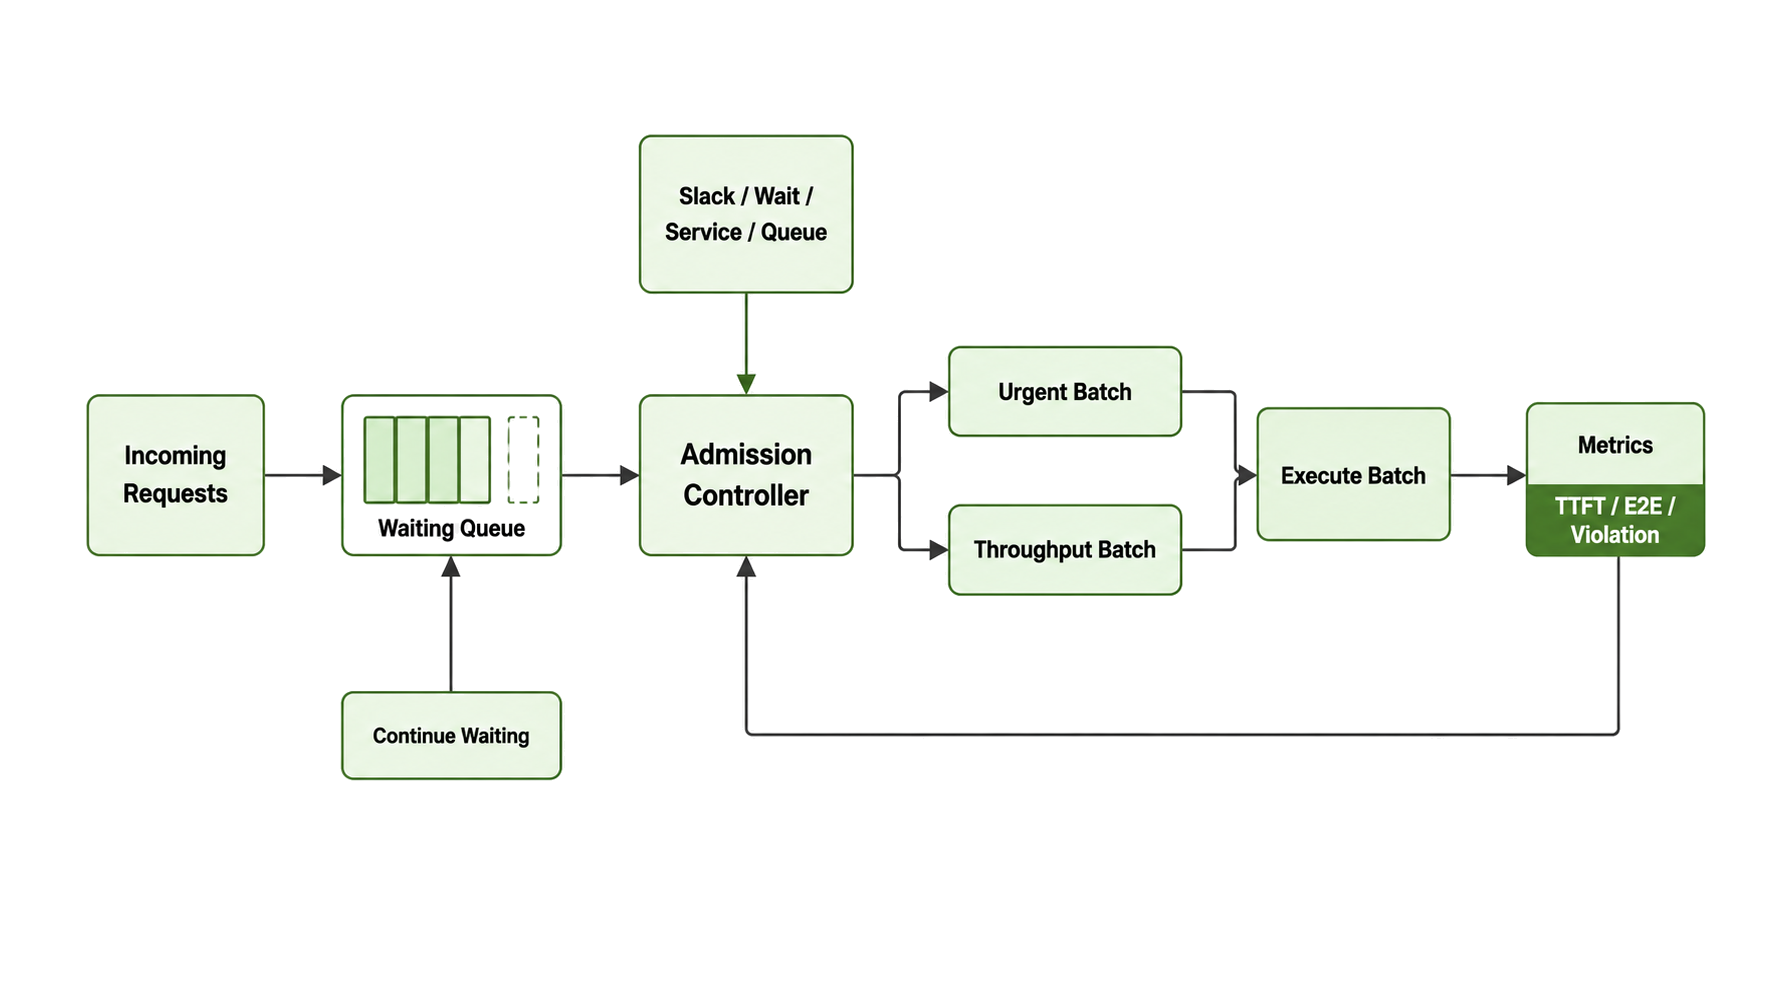
\includegraphics[width=\textwidth]{figures/ch5_2_dynamic_admission_batching.png}
\caption{\textbf{Queue-level Dynamic / Admission Batching 机制示意图}}
\label{fig:ch5-dynamic-admission-batching}
\end{figure}
Incoming Requests 携带 SLO 和 priority 进入 Waiting Queue，Admission Controller 持续读取距离 deadline 的剩余时间、wait time、service estimate 和 queue length。临近 deadline 的请求进入 Urgent Batch，剩余时间较充足的请求进入 Throughput Batch 或继续等待；两个可执行 batch 随后进入 runtime。执行产生的 TTFT、E2E latency 和 SLO violation 由 Metrics 模块反馈给控制器，用于调整 batching window 与 admission threshold。Dynamic batching 会同时改变 batch size、请求组成和等待时间，并围绕各请求的剩余时间预算在线决策。

这类方法的核心思想是把组批从静态规则改为在线决策。调度器可以根据队列长度、请求等待时间、距离 deadline 的剩余时间、prompt 长度、预计输出长度、业务优先级和当前实例负载决定是否立即发起 batch，还是继续等待更多请求。对于剩余时间较充足的请求，可以适当等待以提高吞吐；对于即将违反 TTFT 或 deadline 的请求，应尽快进入执行队列。与 static batching 相比，dynamic batching 的 batch 仍然主要在执行前形成，但形成过程已经具备业务感知能力。

Queue-level Dynamic / Admission Batching 的关键变量包括 batching window、max wait time、admission threshold、request priority、距离 deadline 的剩余时间、estimated service time 和 batch size limit。很多 SLO-aware request batching 工作可以放在这一类中理解：它们并不一定改变 decode iteration 的 active batch 机制，而是先在请求队列和接纳阶段决定谁应该进入下一批执行 \cite{zhang2026jitserve}, \cite{hong2025sola}。

在 CEC 中，dynamic batching 需要把网络时延纳入剩余时间预算。靠近请求入口的实例通常 RTT 较低，但请求池较小；能够聚合多个入口的协作节点请求池更大，但转发距离和排队时间也可能增加。因此，同一个请求应在入口附近立即小批次执行，还是转发到其他协作节点等待更合适的 batch，取决于剩余 SLO、入口到实例链路、当前排队时间和模型能力。Dynamic batching 是 CEC 中自然的业务感知入口，因为它在请求尚未进入长期 decode 循环前就可以完成接纳、排序和路径选择。

Queue-level Dynamic / Admission Batching 的风险在于调度器需要可靠估计请求服务时间。如果输出长度预测错误、队列状态滞后或网络时延估计不准，batching window 和优先级选择可能反而放大尾延迟。因此，在 CEC 中应避免过长等待窗口，并将 admission control、优先级老化和 fallback 策略作为配套机制。
\phantomsection
\subsection*{5.2 Continuous Batching / Iteration-level Batching}
\addcontentsline{toc}{subsection}{5.2 Continuous Batching / Iteration-level Batching}
Continuous Batching 进一步打破了 batch 生命周期。它要解决的是 LLM decode 阶段中请求完成时间不同导致的空槽浪费问题。传统 static 或 dynamic batching 即使在执行前能组成合适 batch，一旦进入自回归 decode，短请求会先完成，长请求还在继续生成。如果 batch 在整个生成过程中固定不变，已完成请求留下的 slot 无法被新请求利用，新到请求也必须等待当前 batch 全部结束。Orca 首先系统化提出 iteration-level scheduling 和 selective batching，成为后续 continuous batching 系统的基础 \cite{yu2022orca}。

当调度边界从请求级下降到 decode iteration 后，batch 的含义就变成图~\ref{fig:ch5-continuous-batching} 中持续变化的 active set。
\begin{figure}[!htbp]
\centering
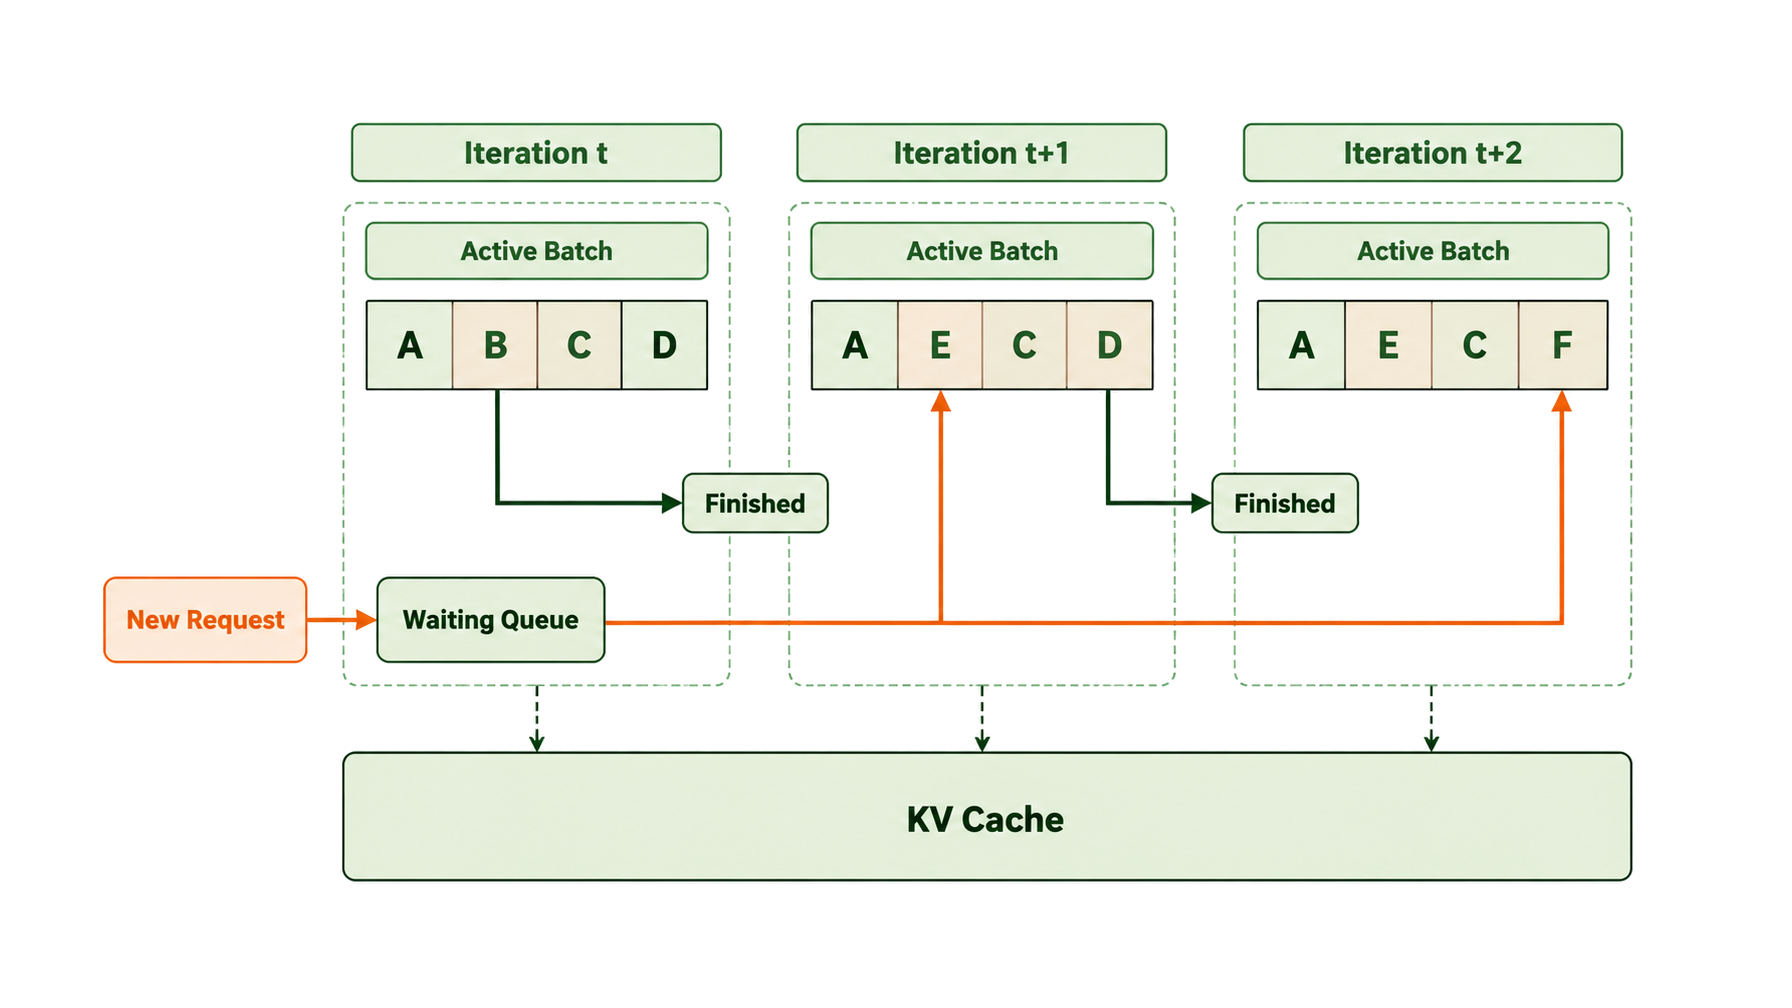
\includegraphics[width=\textwidth]{figures/ch5_3_continuous_iteration_batching.png}
\caption{\textbf{Continuous Batching / Iteration-level Batching 机制示意图}}
\label{fig:ch5-continuous-batching}
\end{figure}
图中每个 Iteration 表示一次 decode iteration，Active Batch 中的四个序列共同生成下一个 token。在 Iteration~\(t\) 结束后，请求 B 完成并退出，请求 E 从 Waiting Queue 加入，因此下一轮的 active set 由 A、B、C、D 变为 A、E、C、D；到 Iteration~\(t+1\) 结束后，请求 D 退出、请求 F 加入，active set 进一步变为 A、E、C、F。A 和 C 连续保留在三个迭代中，其 KV Cache 也持续增长。该过程说明，continuous batching 会在迭代边界及时回收完成请求留下的 slot，并用等待请求补充空位，而不必等待整个 batch 结束。

Continuous Batching 的解决思路，是把 batch 的更新边界缩短到 decode iteration。每生成一轮 token 后，系统都可以移除已经完成的请求，加入完成 prefill 的新请求，或者恢复被抢占的请求。这样 batch 不再是一组固定请求，而是一个随 token 生成持续变化的 active set。Orca 将这一思想形式化为 iteration-level scheduling，使 LLM serving 从“按完整请求批处理”转向“按 token iteration 批处理” \cite{yu2022orca}；FastServe 在这一基础上引入迭代级抢占 \cite{wu2026fastserve}，TokenFlow 面向 streaming token 服务做 preemptive scheduling \cite{chen2026tokenflow}，NanoFlow 则用 nano-batch execution 进一步细化执行流 \cite{zhu2025nanoflow}。

这类方法的核心变量包括 active sequence set、decode batch size、token iteration order、join policy、leave policy、preemption policy、resume policy 和 KV block allocation。由于每轮 decode 都要读取并追加 KV Cache，continuous batching 必须和内存管理绑定：请求能否加入 active batch，不仅取决于是否有计算 slot，也取决于是否有足够 KV block 和状态本地性。vLLM 的 PagedAttention 正是从 KV block 管理角度支撑更大的 active batch 和更低的显存碎片 \cite{kwon2023efficient}；SGLang 用 RadixAttention 复用共享前缀 \cite{zheng2024sglang}；Llumnix 则把运行中请求迁移纳入多实例调度 \cite{sun2024llumnix}。这些工作说明，continuous batching 的 active set 会进一步受到 prefix cache 和实例负载的共同约束。

多租户 LoRA serving 也可以从 continuous batching 角度理解。Punica~\cite{chen2024punica} 和 S-LoRA~\cite{sheng2024slora} 让使用不同 adapter 的序列共享同一个基础模型执行批次，并处理 adapter 权重分页、异构 adapter batching 和定制 LoRA 算子等问题。这些机制决定 batch 内请求能否合并执行，以及合并后的显存和算子开销。

在 CEC 中，Continuous Batching 不能简单照搬云端大请求池策略。靠近请求入口的边缘实例并发通常较低，短时间内能加入 active batch 的请求有限；如果为等待更多 token stream 而延长调度周期，TTFT 会恶化。因此，局部实例更适合短窗口、低等待的 micro-continuous batching，能够聚合多个入口的协作节点则可以形成更稳定的 active batch。对于移动用户，还需要考虑请求是否会在 decode 期间切换入口，避免 active batch 中的 KV 状态和用户路径频繁迁移。

Continuous Batching 是现代 LLM serving 的基础能力，但不是完整的业务感知调度。它提升 decode 阶段资源利用率，却不天然感知 SLO、应用等级、KV 状态迁移、边缘链路和隐私约束。因此，在 CEC 中应把 Continuous Batching 视为 runtime 基座，再叠加 dynamic priority、phase-aware interleaving 和状态感知 admission。
\phantomsection
\subsection*{5.3 Chunked Prefill / Blended Batching}
\addcontentsline{toc}{subsection}{5.3 Chunked Prefill / Blended Batching}
Chunked Prefill / Blended Batching 要解决的是长 prefill 阻塞 decode 的问题。Prefill 处理完整 prompt，矩阵规模大、并行度高，通常更偏 compute-bound；decode 逐 token 生成，频繁访问 KV Cache，更偏 memory-bound 或 latency-bound。如果长 prompt prefill 连续占用 GPU，已经在流式输出的请求会出现 ITL 抖动；如果完全优先 decode，新请求 TTFT 又会被推迟。两阶段混部需要确定 prefill 和 decode 在同一执行资源上的交错方式。Sarathi-Serve~\cite{agrawal2024taming} 将长 prefill 切成 chunks 并与 decode 交错，是这一类方法的代表性工作。

长 prompt 不能直接整段 prefill 的原因，可以通过图~\ref{fig:ch5-chunked-prefill-batching} 看到：系统需要把 prefill chunk 和 decode token 交错安排，在 TTFT 与 ITL 之间控制阶段干扰。
\begin{figure}[!htbp]
\centering
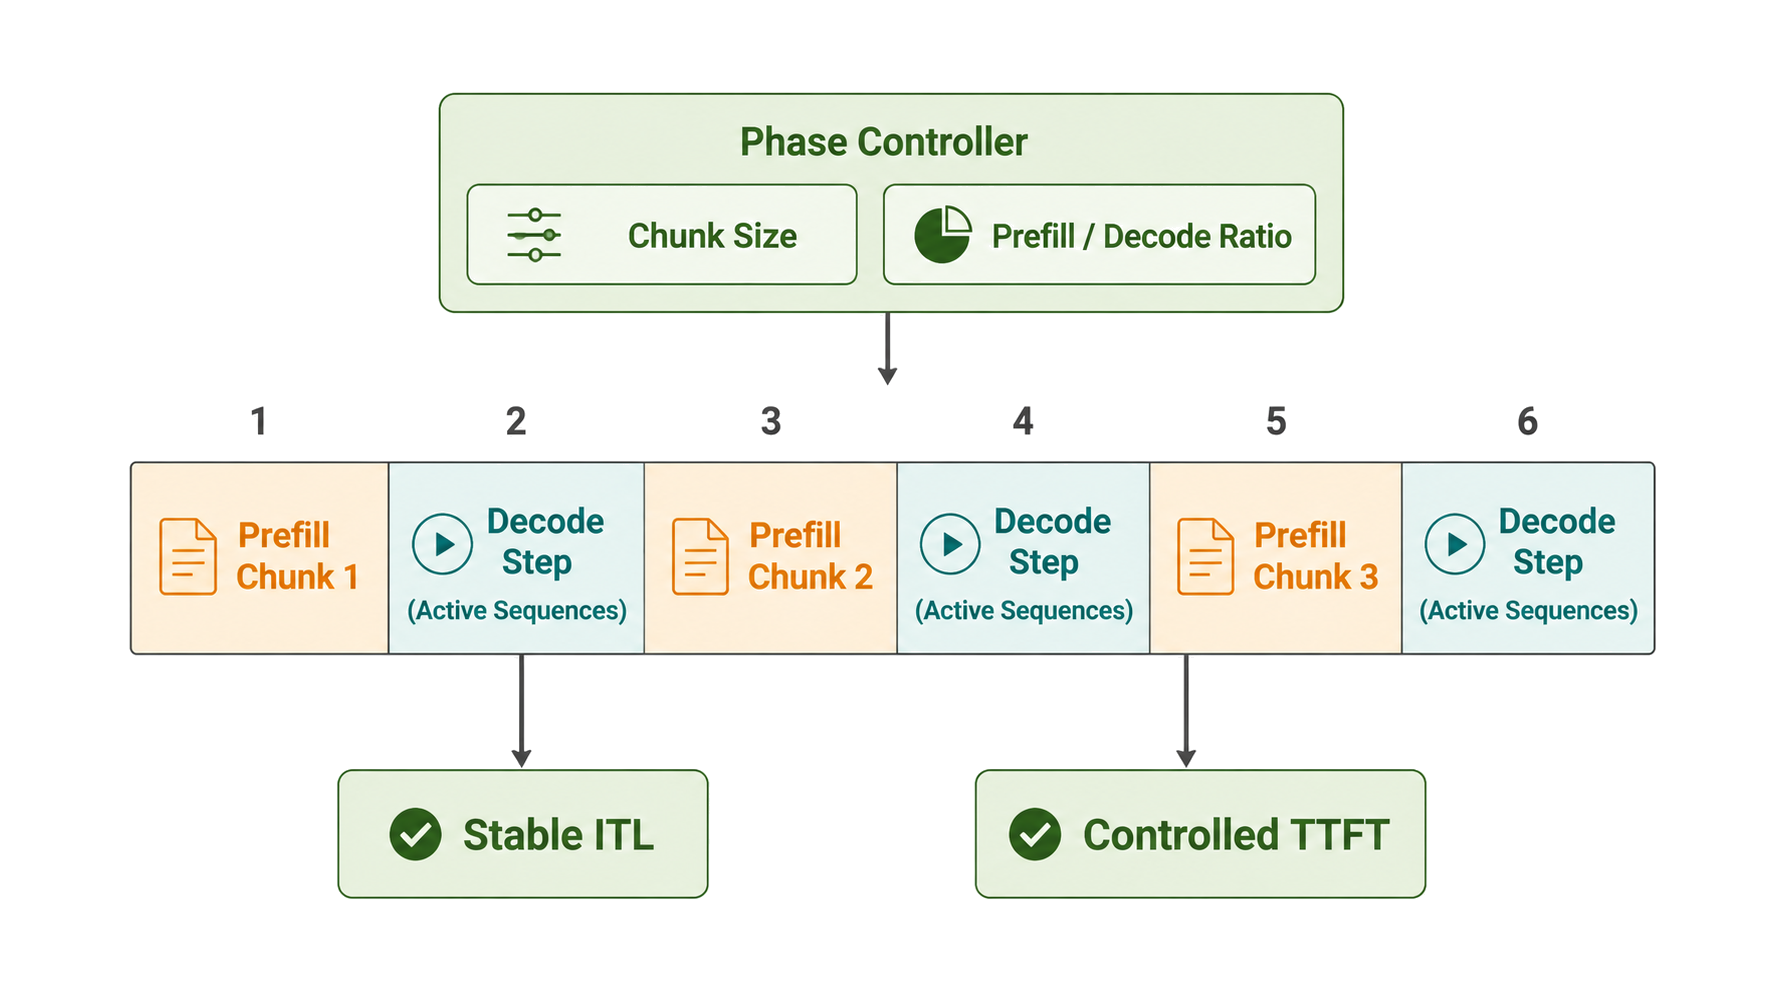
\includegraphics[width=\textwidth]{figures/ch5_4_chunked_prefill_blended_batching.png}
\caption{\textbf{Chunked Prefill / Blended Batching 机制示意图}}
\label{fig:ch5-chunked-prefill-batching}
\end{figure}
图中 Long Prompt 被拆成三个 prefill chunks，并与 Active Sequences 的 decode steps 交替进入六个连续的调度时隙。Phase Controller 通过 chunk size 和 prefill/decode ratio 控制每次执行的 prefill 工作量以及两类阶段的交错频率：chunk 较大时能够提高 prefill 效率，但可能拉长 decode 间隔；chunk 较小时更有利于稳定 ITL，却会增加调度和 kernel 启动开销。因此，该机制通过有限粒度的切块与交错，在保持 decode 流畅性的同时控制新请求的 TTFT。

Chunked Prefill 的思想是把长 prompt 拆成多个 prefill chunk，而不是一次性执行完整 prefill。Blended Batching 则进一步把 prefill chunk 与 decode token 混合在同一个调度周期或同一个 batch 中，使 compute-heavy 的 prefill 和 memory/latency-sensitive 的 decode 交错执行。这样可以平滑每轮计算量，减少长 prefill 对 decode 的阻塞，也能避免 decode 完全占用调度周期导致新请求 TTFT 过高。

这类方法的核心变量包括 chunk size、prefill token budget、decode token budget、prefill-to-decode ratio、interleaving policy、phase quota、online/offline mixing ratio 和 stall control。Chunk 太大，会重新造成 prefill 阻塞；chunk 太小，会增加调度和 kernel overhead。Prefill/decode 比例太偏向 prefill，会伤害 ITL；太偏向 decode，会伤害 TTFT。因此，Chunked Prefill / Blended Batching 的本质是阶段内混合调度和阶段间干扰控制。Libra 可以理解为阶段配额控制的扩展 \cite{ruan2026libra}，NanoFlow 代表更细粒度执行流优化 \cite{zhu2025nanoflow}，LLMStation 和 FlexLLM 则把混合对象扩展到 inference/finetuning co-serving 等更复杂 workload \cite{he2025resource}, \cite{oliaro2026flexllm}。这些工作本质上仍然需要在同一批执行资源上安排不同类型 token 或任务片段的执行顺序。MuxServe 同样涉及 batch scheduling，但其主问题是多模型 serving 的空间共置与时间复用，更适合作为 multi-model multiplexed batching 的横向机制，而不是 chunked prefill 的直接代表 \cite{duan2024muxserve}。

在 CEC 中，这类方法适合由不同能力的边缘节点协同执行。靠近请求入口的节点可以保持较短 decode 间隔，算力更强的协作节点处理较长 prefill chunk；当链路稳定且 KV 传输成本可控时，系统还可以把长 prompt prefill 分配到更强节点，再将可复用状态交给靠近用户的 decode 节点。若链路抖动大或边缘并发不足，过度切分 prefill 可能增加状态传输和调度开销，因此 chunk size 和 interleaving ratio 必须纳入在线代价模型。

Chunked Prefill / Blended Batching 比 continuous batching 更直接处理 prefill/decode 干扰。它适合长 prompt、多轮对话、RAG 增强上下文和流式输出并存的场景，但需要准确控制 chunk size 和阶段配额。对于 CEC，关键是把网络传输和 KV 状态位置纳入阶段混合决策，否则 prefill 拆得越细，跨节点状态交接越可能成为新的瓶颈。
\phantomsection
\subsection*{5.4 Disaggregated Prefill-Decode Batching}
\addcontentsline{toc}{subsection}{5.4 Disaggregated Prefill-Decode Batching}
Disaggregated Prefill-Decode Batching 是对 phase-aware 思路的进一步扩展。Chunked Prefill / Blended Batching 仍然假设 prefill 和 decode 在同一个实例或同一类资源上交错执行；而 disaggregated batching 直接把两阶段拆到不同 worker pool、不同 GPU 实例、不同机器池或不同协作边缘节点。Prefill batch 和 decode batch 分别形成，分别扩缩容，并通过 KV Cache 或中间状态传输衔接。DistServe 从 goodput 优化角度论证阶段解耦 \cite{zhong2024distserve}，Splitwise 强调 prompt pool 与 token pool 的硬件匹配 \cite{patel2024splitwise}，Mooncake 则在 prefill/decode 解耦基础上构建 KVCache-centric serving 架构 \cite{qin2025mooncake}。

PD 分离后的 batching 可以按图~\ref{fig:ch5-disaggregated-pd-batching} 理解：prefill instance 内部形成 prompt batch，decode instance 内部维护 active sequence batch，两个池之间通过 KV/state handoff 连接。
\begin{figure}[!htbp]
\centering
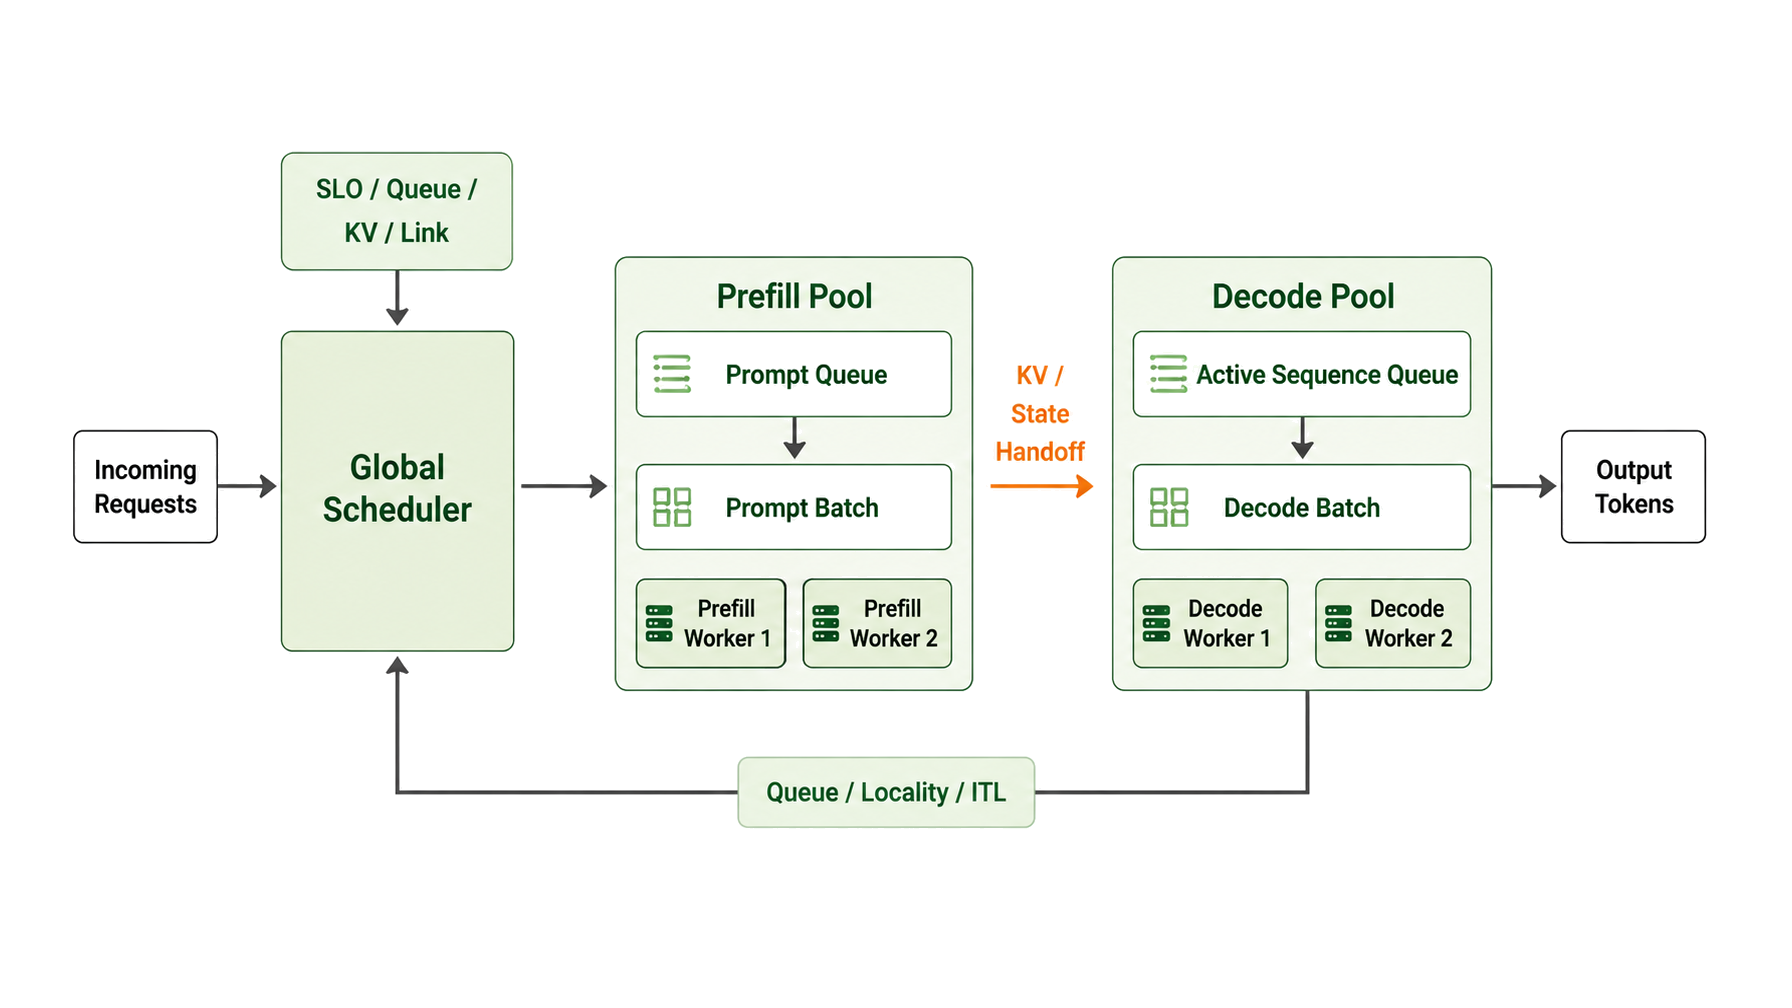
\includegraphics[width=\textwidth]{figures/ch5_5_disaggregated_pd_batching.png}
\caption{\textbf{Disaggregated Prefill-Decode Batching 机制示意图}}
\label{fig:ch5-disaggregated-pd-batching}
\end{figure}
Global Scheduler 根据 SLO、queue length、KV locality 和 link state 将请求送入 Prefill Pool；Prefill Worker 形成 prompt batches 并生成初始 KV blocks。随后 KV / State Handoff 将 KV blocks、state transfer 和 metadata 交给 Decode Pool，Decode Worker 再维护 active sequence batches 并输出 tokens。图中的反馈路径表示 queue length、KV locality、ITL 等运行时指标回流到全局调度器，用于调整后续请求进入哪个 pool 以及是否需要扩缩容。因此，PD 分离后的 batching 实际上变成两个 pool 的独立组批与跨池状态协调问题。

这类方法的出发点是 prefill 和 decode 的计算与访存特征明显不同。Prefill 更偏 compute-bound，适合吞吐导向、更强算力或更大 batch 的资源池；decode 更偏 memory/latency-bound，需要稳定 ITL、低排队和快速状态访问。若两者混部在同一资源池中，长 prefill 可能阻塞 decode，decode 小步迭代又可能降低 prefill 吞吐。Disaggregation 通过物理或逻辑隔离减少两阶段干扰，并允许系统分别为 prefill 和 decode 选择 parallelism、batch size 和扩缩容策略。

Disaggregated Prefill-Decode Batching 的核心变量包括 prefill worker pool、decode worker pool、phase queue、KV transfer、state locality、worker scaling、prefill/decode routing 和 global scheduling。它的收益来自阶段资源匹配和干扰隔离，但代价集中在 KV 传输、状态连续性和跨节点调度。Prefill 完成后，decode 必须访问初始 KV Cache；如果 KV 传输慢、远程访问不稳定或用户入口发生变化，disaggregation 的收益会被状态成本抵消 \cite{zhong2024distserve}, \cite{qin2025mooncake}。

本节关注 PD 分离之后的 batching：prefill pool 如何形成 prompt batch，decode pool 如何维护 active sequence batch，以及两个 pool 之间如何通过 KV/state handoff 协调。

在 CEC 中，disaggregated batching 可以映射到不同能力的协作节点：算力较强或能够聚合请求的节点承担 prefill-heavy 请求，靠近用户且持有会话状态的节点负责低时延 decode；容量较大的节点也可以维护 prefill pool 和 KV state service，其他节点只在需要较低 ITL 时承担 decode。对于移动用户，系统还需要判断 decode worker 是否应该跟随入口迁移，还是远程访问原有 KV。也就是说，CEC 下的 disaggregated batching 不能只看 GPU 利用率，还必须同时看链路稳定性、KV 迁移成本和服务连续性。

Disaggregated Prefill-Decode Batching 适合 prefill/decode 负载差异明显、阶段队列规模足够、状态传输成本可控的场景。若请求很短、边缘并发很低或链路抖动大，复杂阶段拆分可能不如本地 blended batching 稳定。因此，CEC 中应把 disaggregation 视为跨实例的资源组织方式，而不是默认打开的单点优化。
\phantomsection
\subsection*{5.5 面向华为验证环境的方案建议}
\addcontentsline{toc}{subsection}{5.5 面向华为验证环境的方案建议}

异构 Ascend 推理服务中的请求到达率、输入输出长度、KV Cache 占用和距离 deadline 的剩余时间不断变化，合适的 batch size、token budget、等待窗口和请求顺序也会随之改变。固定配置难以覆盖这些组合；普通强化学习虽然能够根据运行状态调整参数，但探索和随机输出可能造成显存越界、关键请求超时或运行时无法执行。为明确动态 batching 在不同请求特征下能够获得多大收益，本文先建立设备、网络、模型和请求的统一系统模型，分析请求长度与 batch size 变化时相对 Static-FIFO 的性能范围。该结果一方面刻画动态组批可利用的优化空间，另一方面为后续强化学习的状态、动作和优化目标设计提供依据。在此基础上，本文提出带拉格朗日约束和运行时安全投影的 Safe-RL batching 方法。

评价时先检查 SLA 和运行安全，再比较性能。对同一模型、请求轨迹和硬件环境，只有 P90/P99 TTFT、TPOT 和 E2E latency 满足业务配置，显存保持在可用范围内，且受控实验中未发生 OOM、不可执行动作和已接纳关键请求硬超时，该运行点才进入完成请求速率与平均 E2E latency 的比较。实验目标是相对 Static-FIFO 将满足 SLA 的请求处理速度提高 20\%，平均 E2E latency 下降 20\%，并保持零硬违规 \cite{huawei2026internal}。

为估计动态组批在验证环境中的性能空间，本文选取四卡 A800T-A2、100~Gbps 直连场景，CodeLlama34B 和 Qwen2-VL-7B-Instruct 沿用第四章得到的非均匀 PP 部署，并让输入和输出覆盖短、中、长三档。具体设备算力、layer 分配和请求长度设置将在后文给出。

理论分析中的 Static-FIFO 使用固定 batch size 和等待窗口，按请求到达顺序形成批次，并在当前批次完成后再处理下一批。批内输入按最长 prompt 补齐，生成过程持续到最长输出结束。极端情况下，一个 batch 包含 1 个最长请求和 63 个最短请求，短请求会承担大量额外计算。用 Static-FIFO 的总计算量除以所有请求各自所需计算量之和，再减 1，得到 \textbf{CodeLlama34B 和 Qwen2-VL-7B-Instruct 的计算侧提升上界分别为 1060.2\% 和 353.9\%}，该上界属于理论上界，实际部署中达不到。

为了在训练 Safe-RL 前先观察长度感知组批能够获得的大致收益，本文进一步采用一个长度相近组批算法：每次观察队首 24 个等待请求，选择距离 TTFT deadline 最近的请求作为基准；当紧迫程度相同时，优先选择到达时间最早的请求。算法再根据预计的 prefill 和 decode 计算量对其余请求排序，选择执行开销最接近的 7 个请求组成大小为 8 的 batch。\textbf{与 Static-FIFO 相比，该算法在 CodeLlama34B 和 Qwen2-VL-7B-Instruct 上的预估提升分别为 111.9\% 和 90.1\%}。这一结果用于判断动态调整请求组合是否具有足够的优化空间，最终收益仍需在显存、请求到达顺序和 SLA 约束下通过 Safe-RL 实验验证 \cite{huawei2026internal}。

\subsubsection*{5.5.1 系统模型}
\addcontentsline{toc}{subsubsection}{5.5.1 系统模型}

Batching 控制依赖请求、模型、部署资源和运行状态四类信息。为了统一描述算法能够观察和控制的对象，系统模型进一步给出由模型计算量、设备算力和链路开销推导 prefill、decode 服务时间的方法。图~\ref{fig:ch5-system-model} 左侧给出验证环境中的异构设备拓扑：E1 和 E2 使用同一组四台 A800T-A2，其中两台使用完整算力，另外两台分别使用一半和四分之一算力，并分别考察 100~Gbps 直连和 25~Gbps RDMA；E3 使用 56~GB/s HCCS 连接两台设备；E4 则通过 25~Gbps 链路连接 310P、半算力 910B4 和完整算力 910B4。中间部分将 PP stage、请求特征和运行状态映射到这些设备，并据此计算 prefill、decode、排队和显存开销。右侧在统一服务时间模型上分析不同请求长度与 batch size 下相对 Static-FIFO 的性能范围，并给出在线 batching 需要调节的参数及评价指标。这些信息随后作为 Safe-RL 的状态与性能反馈。

\begin{figure}[!htbp]
\centering
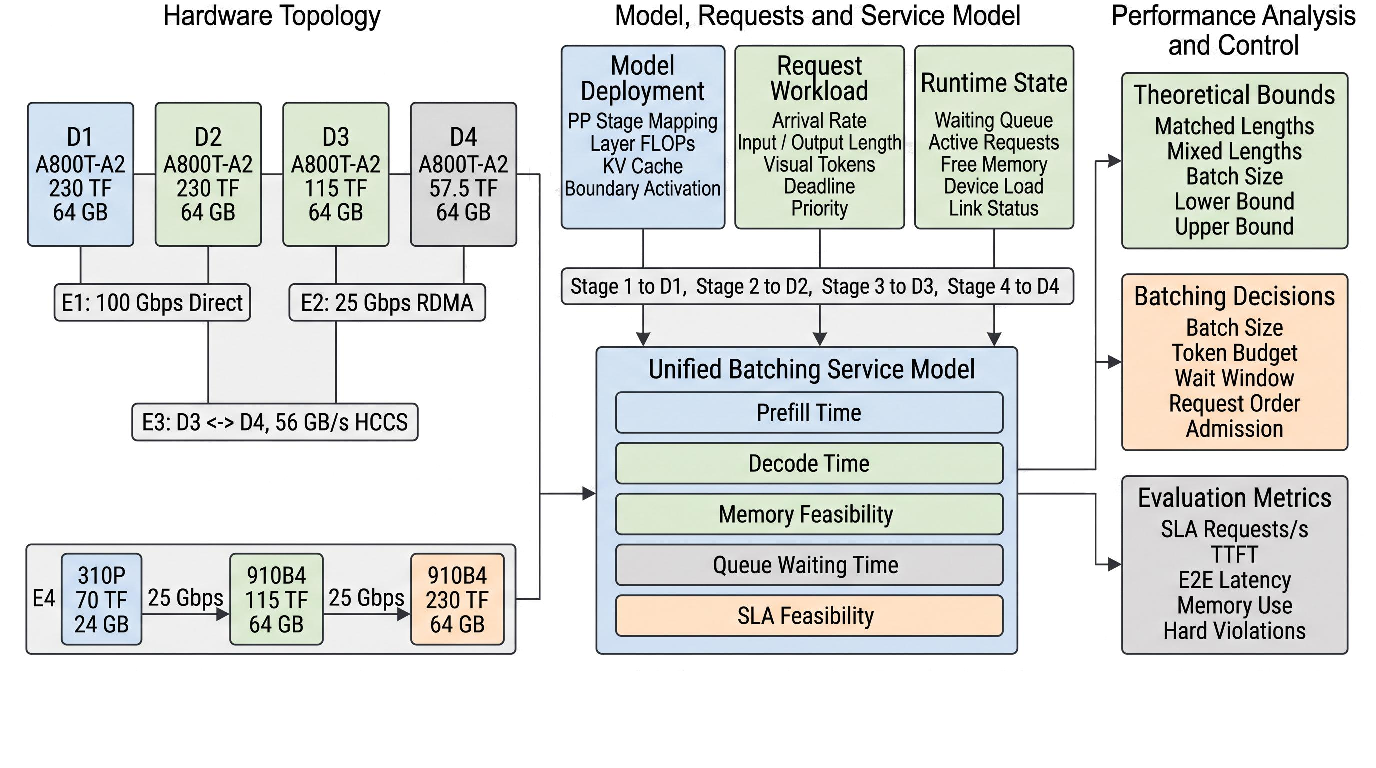
\includegraphics[width=\textwidth]{figures/ch5_system_model.pdf}
\caption{面向异构设备的业务感知 batching 系统模型}
\label{fig:ch5-system-model}
\end{figure}

硬件环境表示为图 \(\mathcal H=(\mathcal V,\mathcal E)\)。设备节点 \(g\in\mathcal V\) 记录当前可用算力 \(F_g\)、可用显存 \(M_g\) 和运行状态，链路 \((g,g')\in\mathcal E\) 记录有效带宽 \(B_{g,g'}\) 与固定传输时延 \(L_{g,g'}\)。模型沿用第四章确定的非均匀 PP 部署方案 \(\mathcal D\)，其中包含各 stage 的放置设备、连续 layer 边界以及相邻 stage 之间的 activation 传输路径。对于 stage \(k\)，其有效算力记为 \(F_k^{\mathcal D}\)，prefill 与 decode 的实测计算效率分别记为 \(\eta_{k}^{\mathrm{pre}}\) 和 \(\eta_{k}^{\mathrm{dec}}\)。

到达系统的请求 \(r_i\) 由到达时间 \(a_i\)、文本输入长度 \(P_i\)、visual token 数 \(V_i\)、预测输出长度 \(\widehat O_i\)、实际输出长度 \(O_i\)、请求 deadline \(d_i\) 和业务优先级 \(\kappa_i\) 描述。纯文本请求令 \(V_i=0\)。实际输出长度 \(O_i\) 在请求完成后用于评价预测误差和服务结果，在线决策只能读取 \(\widehat O_i\)。控制器在每个决策窗口读取等待队列、active requests、各请求的剩余时限、近期到达率、KV Cache 占用、剩余显存和设备利用率，并决定下一窗口的组批参数与请求顺序。

模型计算量直接由网络结构和请求长度得到。设一个文本 Transformer layer 的参数量为 \(N_{\mathrm{layer}}\)，hidden size 为 \(h\)。长度为 \(P\) 的单请求 prefill 计算量和生成 \(O\) 个 tokens 的 decode 计算量分别为
\[
C_{\mathrm{pre}}(P)=
\sum_{l=1}^{L}\left(2PN_l+4P^2h_l\right),
\]
\[
C_{\mathrm{dec}}(P,O)=
\sum_{u=1}^{O}\sum_{l=1}^{L}
\left(2N_l+4(P+u)h_l\right).
\]
第一式中的线性项来自模型参数参与的矩阵计算，二次项来自 prefill attention；第二式逐 token 累加 decode 计算。CodeLlama34B 使用 48 个文本 layers 的参数。Qwen2-VL-7B-Instruct 还要加入视觉编码器和模态投影的计算量，并把文本 decoder 的上下文长度写为 \(P+V\)。因此，图像数量、分辨率和预处理后 visual token 数会同时影响 prefill 时间与后续 decode 的上下文长度。

对部署 \(\mathcal D\) 中的 stage \(k\)，batch 的 prefill 服务时间由该 stage 承担模块的 FLOPs、有效算力和通信共同计算：
\[
T_{k}^{\mathrm{pre}}(b,P,V)=
\frac{C_{k}^{\mathrm{pre}}(b,P,V)}
{\eta_{k}^{\mathrm{pre}}F_k^{\mathcal D}}\times10^3
+T_{k}^{\mathrm{link,pre}}.
\]
单轮 decode 时间 \(T_{k}^{\mathrm{dec}}(b,P,V,u)\) 采用相同形式，其中计算量对应当前 token 步 \(u\)。对单个请求，完整 prefill 时间和生成 \(O\) 个 tokens 的 decode 时间分别为
\[
T_{\mathcal D}^{\mathrm{pre}}=\sum_k T_k^{\mathrm{pre}},
\qquad
T_{\mathcal D}^{\mathrm{dec}}=\sum_{u=1}^{O}\sum_k T_k^{\mathrm{dec}}(u).
\]
各量均以 FLOPs、FLOPs/s 和 ms 为单位。第四章已经选择纯 PP，因此式中的通信项只包含相邻 stages 之间的 activation 传输。部署前令计算效率系数为 1，可得到由模型规格、设备有效算力和链路共同确定的时间参照；进入 Ascend 环境后，以不同 batch size 和长度下的逐层执行时间以及 CANN/HCCL 通信时间更新效率和通信项。由此形成的 prefill/decode 服务时间曲线直接用于 SLA 仿真和 Safe-RL 训练。

显存约束同时计入模型权重、activation、KV Cache 和运行时预留。设 batch 中 active requests 的当前上下文长度为 \(\ell_i\)，单 token KV Cache 大小为 \(m_{\mathrm{KV}}\)，则 KV 占用近似为 \(m_{\mathrm{KV}}\sum_i\ell_i\)。该值与各 stage 已驻留权重和运行时空间共同决定当前能够接纳的请求数及 token budget。

\subsubsection*{5.5.2 性能理论分析}
\addcontentsline{toc}{subsubsection}{5.5.2 性能理论分析}

在统一系统模型下，本文以 Static-FIFO 为基线，先分析不同请求组合产生的长度补齐计算，再判断在线算法能够减少其中多少开销。当一个最长请求与其余最短请求进入同一 batch 时，Static-FIFO 的冗余计算最多，对应所考察请求范围内的计算侧提升上界。在此基础上，有限窗口长度感知算法给出受到观察范围和请求顺序限制时的可实现预估，进一步改变 batch size 还可以分析批内请求数量对两类结果的影响。这些结果为 Safe-RL 选择需要观察的请求特征、需要调节的 batching 参数以及合理的性能目标提供理论依据；SLA、排队、KV Cache 和控制开销的影响则在 5.5.6 节通过请求轨迹实验验证。

对于请求 \(r_i\)，将完成其 prefill 和 decode 所需的模型计算量记为
\[
C_i=C_{\mathrm{pre}}(P_i,V_i)+C_{\mathrm{dec}}(P_i,V_i,O_i).
\]
下文用 \(C(P,V,O)\) 表示具有给定输入、视觉和输出长度的请求计算量，因此 \(C_i=C(P_i,V_i,O_i)\)。
设一个静态 batch 包含 \(B\) 个请求。若执行过程按 batch 内最长输入和最长输出进行长度补齐（padding），记 \(P_{\max}\)、\(V_{\max}\) 和 \(O_{\max}\) 为该 batch 的最大长度，则总计算量近似为
\[
W_{\mathrm{pad}}=
B\,C(P_{\max},V_{\max},O_{\max}).
\]
当长度相近的请求被放在一起，并且短请求结束后空出的执行位置能够及时回收时，请求集合至少要完成的有效计算量为
\[
W_{\mathrm{use}}=\sum_{i=1}^{B}C_i.
\]
两者的比值
\[
S_{\mathrm{len}}=\frac{W_{\mathrm{pad}}}{W_{\mathrm{use}}}
\]
给出长度重排在该简化模型中的计算侧速度倍数上界。相对 Static-FIFO 的提升为 \((S_{\mathrm{len}}-1)\times100\%\)。\(S_{\mathrm{len}}\) 是无量纲的速度倍数；实际 requests/s 由服务时间模型或硬件实测得到，并进一步接受显存、排队和 deadline 检查。

表~\ref{tab:ch5-model-workload} 给出代表性请求的模型计算量和部署前服务时间。CodeLlama34B 采用 512-token 输入和 256-token 输出；Qwen2-VL-7B-Instruct 采用 640 个 visual tokens、1024 个 text tokens 和 256-token 输出。时间计算使用第四章 E1 场景中选出的 PP 部署，CodeLlama34B 的文本层分配为 \((18,18,9,3)\)，Qwen2-VL-7B-Instruct 为 \((4,14,7,3)\)。计算同时计入各 stage 的有效算力和 100~Gbps 链路上的边界 activation 传输，batch size 取 1，计算效率系数取 1。

\begin{table}[!htbp]
\centering
\small
\setlength{\tabcolsep}{5pt}
\renewcommand{\arraystretch}{1.18}
\caption{代表性请求的模型计算量与 E1 部署前服务时间}
\label{tab:ch5-model-workload}
\begin{tabularx}{\textwidth}{>{\raggedright\arraybackslash}X>{\centering\arraybackslash}m{0.15\textwidth}>{\centering\arraybackslash}m{0.15\textwidth}>{\centering\arraybackslash}m{0.17\textwidth}>{\centering\arraybackslash}m{0.17\textwidth}}
\hline
模型与请求配置 & Prefill / TFLOPs & Decode / TFLOPs & Prefill / ms & Decode / ms \\
\hline
CodeLlama34B，512 / 256 tokens & 34.43 & 17.27 & 207.84 & 104.23 \\
Qwen2-VL-7B-Instruct，640 visual + 1024 text / 256 output & 27.19 & 3.53 & 177.78 & 24.53 \\
\hline
\end{tabularx}
\end{table}

表中的时间用于把 FLOPs 计算与具体设备、链路联系起来。实际 batch size 增大后，将批内所有请求的 FLOPs 和 activation 大小代入同一公式即可得到对应服务时间。Ascend kernel 的实际利用率通常随 batch size 和序列长度变化，因此正式实验以逐层测量得到的 \(\eta_k^{\mathrm{pre}}\)、\(\eta_k^{\mathrm{dec}}\) 和通信时间替换部署前参照，再判断 TTFT、TPOT 和 E2E latency 是否满足 SLA。

对任一 batching 配置 \(a\)，将其 batch size、请求长度和执行顺序代入服务时间曲线，可以得到完成该批请求所需的时间 \(\widehat T(a)\)，并进一步估计各请求的等待时间、TTFT 和 E2E latency。记 \(\mathcal A_{\mathrm{SLA}}\) 为同时满足显存限制和 SLA 阈值的配置集合，\(B(a)\) 为配置 \(a\) 完成的请求数，则部署前的 SLA 吞吐上界写为
\[
R_{\mathrm{SLA}}^{\mathrm{ub}}=
\max_{a\in\mathcal A_{\mathrm{SLA}}}
\frac{B(a)\times10^3}{\widehat T(a)}
\quad \mathrm{requests/s}.
\]
输入长度和 visual token 数主要改变 prefill 时间，输出长度改变 decode 轮数，batch size 同时影响计算效率、KV Cache 和等待时间，因此这些参数都会改变可行配置集合与吞吐上界。正式实验使用 Ascend 实测服务时间重新计算 \(\widehat T(a)\)，并通过请求轨迹验证预测的 SLA 可行性。

理论上界用于界定请求重排的最大优化空间，可实现的部署前预估则由有限窗口长度感知组批得到。每次准备新 batch 时，调度器观察等待队列前 \(W\) 个请求，先选择剩余 TTFT 时间最短的请求作为本批的基准请求，以避免长度匹配导致紧急请求继续等待；随后利用 5.5.1 节的服务时间模型估计其余请求的 prefill 和 decode 执行开销，从中选择预计执行开销最接近的 \(B-1\) 个请求。请求加入后还要单独检查 KV Cache、显存和 SLA，检查失败时跳过该请求并继续考察下一个。部署前分析以 \(B=8\) 为参考 batch size，并令观察范围为其三倍，即 \(W=24\)；后续再改变 \(W\) 和 \(B\) 检查结果的敏感性。

为了在相同计算口径下比较理论空间与有限窗口算法，记 Static-FIFO 形成的所有 batches 的长度补齐计算量为 \(W_{\mathrm{FIFO}}\)，全部请求自身所需的有效计算量为 \(W_{\mathrm{use}}\)，有限窗口长度感知算法形成的 batches 的长度补齐计算量为 \(W_{\mathrm{len}}\)。处理相同数量请求时，两种提升分别为
\[
G_{\mathrm{ub}}=\frac{W_{\mathrm{FIFO}}}{W_{\mathrm{use}}}-1,
\qquad
G_{\mathrm{len}}=\frac{W_{\mathrm{FIFO}}}{W_{\mathrm{len}}}-1.
\]
其中，\(G_{\mathrm{ub}}\) 表示完全消除额外长度补齐计算时的上界，\(G_{\mathrm{len}}\) 表示在 \(W=24\)、\(B=8\) 条件下执行上述排序算法得到的预估提升。两者均使用 5.5.1 节的模型 FLOPs 计算，不再使用输入输出 token 数的线性加权值。

表~\ref{tab:ch5-length-aware-estimate} 使用短、中、长三档请求进行计算。CodeLlama34B 的输入长度为 128、512 和 2048 tokens，Qwen2-VL-7B-Instruct 的文本输入长度为 256、1024 和 4096 tokens，并固定 640 个 visual tokens；输出长度均为 64、256 和 512 tokens。计算侧预估令同一观察窗口中的请求均已到达且 SLA 紧迫程度相同，因而只比较长度补齐计算量；请求到达和 deadline 的影响在随后请求轨迹中加入。

\begin{table}[!htbp]
\centering
\small
\setlength{\tabcolsep}{4pt}
\renewcommand{\arraystretch}{1.18}
\caption{短、中、长三档随机请求下的纯计算上界与有限窗口排序预估}
\label{tab:ch5-length-aware-estimate}
\begin{tabularx}{\textwidth}{>{\raggedright\arraybackslash}X>{\centering\arraybackslash}m{0.16\textwidth}>{\centering\arraybackslash}m{0.16\textwidth}>{\centering\arraybackslash}m{0.16\textwidth}>{\centering\arraybackslash}m{0.16\textwidth}}
\hline
请求分布 & \multicolumn{2}{c}{CodeLlama34B} & \multicolumn{2}{c}{Qwen2-VL-7B-Instruct} \\
 & 计算上界 & 排序预估 & 计算上界 & 排序预估 \\
\hline
输入输出长度一致 & 0.0\% & 0.0\% & 0.0\% & 0.0\% \\
仅输入长度变化 & 135.5\% & 115.3\% & 103.1\% & 89.5\% \\
仅输出长度变化 & 35.7\% & 32.8\% & 11.8\% & 11.0\% \\
输入输出长度同时变化 & 173.3\% & 111.9\% & 115.7\% & 90.1\% \\
\hline
\end{tabularx}
\end{table}

输入长度变化带来的提升高于输出长度变化，主要原因是较长 prompt 会同时增加参数计算和 attention 计算，并把静态 batch 中其它短请求的 prefill 长度一并抬高。表中的有限窗口排序只能观察队首 24 个请求，因此预估结果低于可以在全部请求中自由匹配的计算上界；加入真实到达时间和 deadline 后，紧急请求优先还会进一步限制长度匹配空间。在输入输出长度同时变化时，CodeLlama34B 的纯计算上界为 173.3\%，有限窗口排序预估为 111.9\%；Qwen2-VL-7B-Instruct 的两项结果分别为 115.7\% 和 90.1\%。这些数值用于描述组批算法自身能够减少多少长度补齐计算，尚未计入请求等待、显存限制和 SLA 筛选。

将上述规则应用于带到达时间、输入输出长度和 deadline 的请求轨迹后，可以得到实际形成的 batch 序列。每个 batch 的完成时间由 \(\widehat T(a)\) 计算，请求等待时间由到达时刻与 batch 启动时刻之差得到。设轨迹持续时间为 \(T_{\mathrm{trace}}\)，单位为 s，其中满足 SLA 并完成的请求数为 \(N_{\mathrm{SLA}}\)，则该规则的预估请求处理速度为
\[
\widehat R_{\mathrm{len}}=
\frac{N_{\mathrm{SLA}}}{T_{\mathrm{trace}}}
\quad \mathrm{requests/s}.
\]
在相同请求轨迹上运行 Static-FIFO，即可由 \(\widehat R_{\mathrm{len}}/\widehat R_{\mathrm{FIFO}}-1\) 得到长度感知组批的预估提升。该结果反映有限观察范围、请求到达顺序和 SLA 共同约束下能够实现的参考性能，并作为 Safe-RL 设计与实验结果之间的中间参照。

为了观察极端长度失配对计算上界的影响，进一步使用 \(B=64\) 的请求集合进行比较。CodeLlama34B 的输入长度取 128、512 和 2048 tokens，Qwen2-VL-7B-Instruct 取 256、1024 和 4096 text tokens，并固定 640 个 visual tokens；输出长度取 64、256 和 512 tokens。对 decode 而言，长度匹配最好的情况是 64 个请求具有相同的输出 token 数；同时计入 prefill 后，还要求输入长度一致，此时没有额外的长度补齐计算。输出失配场景由 1 个 512-token 输出和 63 个 64-token 输出组成，输入失配场景由 1 个最长输入和 63 个最短输入组成。本文将“1 个最长输入、最长输出请求与 63 个最短输入、最短输出请求”定义为组合失配的最差情况。表~\ref{tab:ch5-batching-extreme-bound} 给出这些极端组合下的纯计算上界。

\begin{table}[!htbp]
\centering
\small
\setlength{\tabcolsep}{4pt}
\renewcommand{\arraystretch}{1.18}
\caption{64 个请求极端长度组合下的纯计算上界}
\label{tab:ch5-batching-extreme-bound}
\begin{tabularx}{\textwidth}{>{\raggedright\arraybackslash}X>{\centering\arraybackslash}m{0.20\textwidth}>{\centering\arraybackslash}m{0.20\textwidth}>{\raggedright\arraybackslash}X}
\hline
请求组成 & CodeLlama34B 上界 & Qwen2-VL 上界 & 含义 \\
\hline
输入输出长度完全一致 & 0.0\% & 0.0\% & 静态组批已无长度补齐损失 \\
仅输出长度极端失配 & 76.1\% & 21.7\% & 长输出持续占用 batch 执行周期 \\
仅输入长度极端失配 & 478.6\% & 280.8\% & 最长 prompt 放大整个 batch 的 prefill 计算 \\
输入输出同时极端失配 & 1060.2\% & 353.9\% & 长输入与长输出的影响叠加 \\
\hline
\end{tabularx}
\end{table}

输入长度带来的范围明显大于输出长度，主要原因是 prefill attention 中包含随输入长度平方增长的计算项。Qwen2-VL 的视觉编码开销对每个请求都存在，因而长度失配占总计算量的比例低于 CodeLlama34B。组合失配中的大幅提升描述 1 个最长请求与 63 个最短请求被强制放入同一静态 batch 的极端情况，用于界定算法层面的最大空间；在线策略还要服从到达顺序、deadline、显存和等待时间限制。

batch size 越大，一个极长请求影响的其它请求越多。表~\ref{tab:ch5-batchsize-bound} 固定组合失配模式，比较不同 \(B\) 下的理论上界。

\begin{table}[!htbp]
\centering
\small
\setlength{\tabcolsep}{7pt}
\renewcommand{\arraystretch}{1.18}
\caption{batch size 对组合失配理论上界的影响}
\label{tab:ch5-batchsize-bound}
\begin{tabular}{c c c}
\hline
Batch size / requests & CodeLlama34B 提升 & Qwen2-VL 提升 \\
\hline
8  & 432.7\% & 225.8\% \\
16 & 671.0\% & 288.4\% \\
32 & 893.1\% & 329.7\% \\
64 & 1060.2\% & 353.9\% \\
\hline
\end{tabular}
\end{table}

较大的 batch 为长度重排提供更多空间，也会增加 KV Cache、单轮执行时间和 TTFT 风险。表中的上界用于界定长度重排的优化空间，Safe-RL 的实际收益还受到可观察请求数、SLA 允许的等待时间、显存和运行时开销影响。算法在这些条件下联合调整 batch 容量、token budget 与请求顺序。进入硬件环境后，再使用 Ascend 实测的 prefill 和 decode 服务时间校准理论结果。

\subsubsection*{5.5.3 基于安全强化学习的 Batching 算法}
\addcontentsline{toc}{subsubsection}{5.5.3 基于安全强化学习的 Batching 算法}

前述理论分析表明，请求长度、batch size 和可观察请求范围都会改变 batching 的优化空间；在线系统还要同时处理到达率、KV Cache、deadline、prefill/decode 干扰和运行时能力。若为这些变量逐项设置阈值，规则数量会快速增加，并且一次调整对后续队列和显存的影响难以由局部规则评价。强化学习能够从连续运行反馈中学习多变量之间的关系，因此适合用于动态 batching 控制。

现有系统已经提供了必要的执行基础。Orca \cite{yu2022orca} 支持迭代级调度，vLLM \cite{kwon2023efficient} 提供灵活的 KV Cache 管理，Sarathi-Serve \cite{agrawal2024taming} 和 DistServe \cite{zhong2024distserve} 分别利用 chunked prefill 与 prefill/decode 分离缓解阶段干扰，JITServe \cite{zhang2026jitserve} 和 SOLA \cite{hong2025sola} 进一步考虑 deadline。这些机制扩大了可调节的参数和执行方式，也使固定规则更难覆盖全部组合。

普通强化学习策略在训练探索、负载突变和状态估计误差下可能输出越界动作。本文采用 Safe-RL 将长期风险约束与当前窗口的确定性安全检查结合起来。Actor 根据请求、资源和 SLA 状态提出 batching 方案，Critic（价值评估网络）根据后续运行结果评价该方案的长期完成请求数与风险；拉格朗日约束用于限制多个窗口上的累计风险，安全投影在动作下发前检查显存、deadline 和运行时支持范围。无法修正的动作回退到最近的稳定配置。

图~\ref{fig:ch5-batching-architecture} 给出了完整闭环。系统先采集队列、请求长度、KV Cache 和 SLA 状态，Actor 输出 batch 参数、请求排序和执行机制，安全投影生成可执行配置，推理运行时返回完成请求数、时延、资源占用和违规事件，反馈再用于更新 Actor、Critic 和约束模型。该方法的重点是在动态提高完成请求速度的同时，使受控压力实验中的 OOM、不可执行动作和已接纳关键请求硬超时均保持为 0。

\begin{figure}[!htbp]
\centering
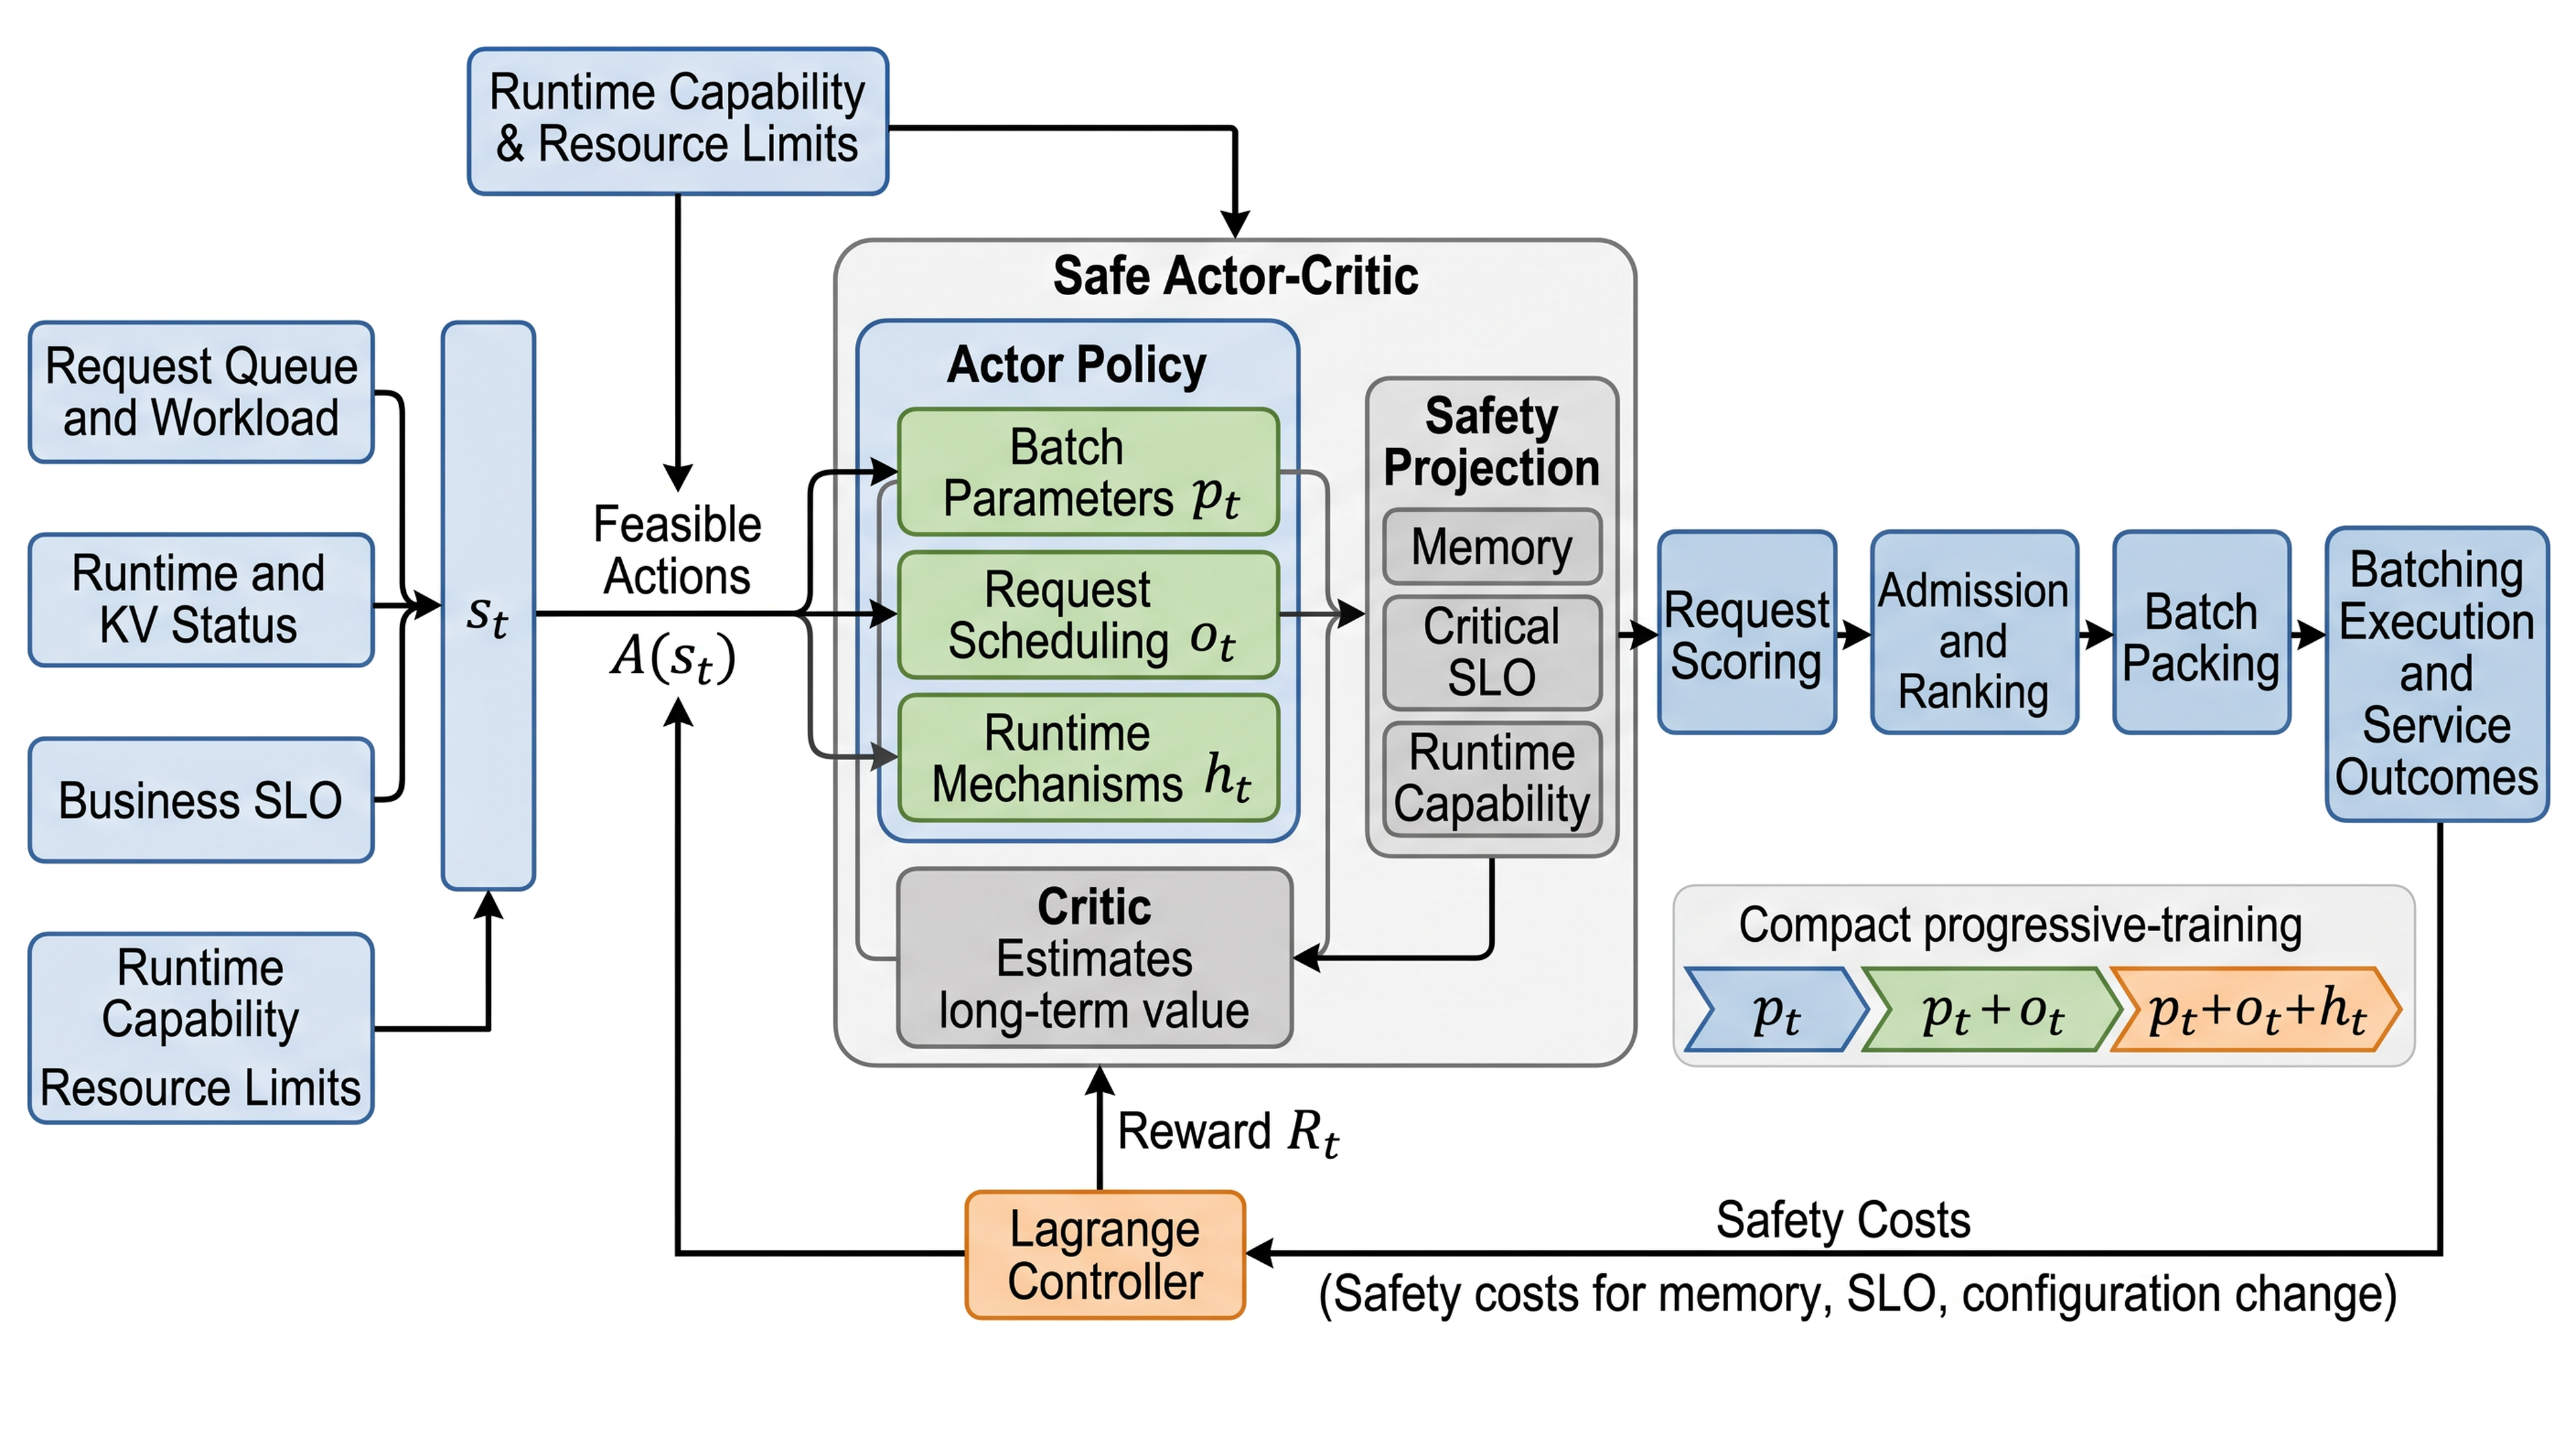
\includegraphics[width=0.88\textwidth]{figures/ch5_safe_rl_batching.png}
\caption{基于拉格朗日约束和安全投影的在线 batching 优化架构}
\label{fig:ch5-batching-architecture}
\end{figure}

\subsubsection*{5.5.4 CMDP 建模与决策生成}
\addcontentsline{toc}{subsubsection}{5.5.4 CMDP 建模与决策生成}

连续 batching 控制可以写成约束马尔可夫决策过程（Constrained Markov Decision Process，CMDP）。这一模型描述一次配置调整对后续队列、KV Cache 和请求时限的持续影响，并进一步规定 Actor 的输出如何转换为实际 batch，使各项决策都有明确的数据来源和运行时取值范围。

本文将推理过程划分为控制窗口 \(t=0,1,\ldots\)，每个窗口依次完成状态采集、动作生成、运行执行和反馈更新。CMDP 表示为
\[
\mathcal M=(\mathcal S,\mathcal A,\mathcal P,R,\{\xi^j\},\gamma),
\]
其中，\(\mathcal S\) 和 \(\mathcal A\) 分别为状态空间与动作空间，\(\mathcal P\) 描述执行动作后的状态变化，\(R\) 表示服务收益，\(\xi^j\) 表示第 \(j\) 类运行风险，\(\gamma\) 用于降低较远反馈对当前决策的影响。

窗口开始时的状态记为 \(s_t=(q_t,z_t,d_t)\)。\(q_t\) 包含等待队列、active requests、prefill/decode 请求数、近期到达率和输入输出长度分布；\(z_t\) 包含可用显存、剩余 KV blocks、设备利用率、近期服务时间、链路状态、上一窗口配置和运行时支持能力；\(d_t\) 包含请求优先级、deadline 及其剩余时间。模型结构、单 token KV Cache 大小和 5.5.1 节得到的 prefill/decode 服务时间曲线作为相对稳定的上下文输入。

动作 \(a_t\) 包含三类决策。第一类是 batch 容量参数，包括 active batch 上限 \(b_t\)、token budget \(u_t\)、最大等待窗口 \(w_t\)、prefill chunk size \(c_t\) 和 prefill/decode 配额 \(\rho_t\)。第二类是请求调度参数，包括准入阈值 \(\tau_t\) 与请求排序权重 \(\vec{\omega}_t\)。第三类是运行时机制 \(h_t\)，用于选择当前环境已经支持的 chunked prefill、长请求隔离或 PD 资源池路由。容量参数和调度参数在短周期更新，切换开销较高的机制在较长周期更新。

这些决策变量由运行状态逐步生成。系统先读取 Ascend 推理运行时支持的参数、取值范围和调整粒度；再依据实例并发上限、剩余 KV blocks 和单 token KV 增量确定 \(b_t\) 与 \(u_t\) 的上界，依据 deadline、队列积压和到达率限制 \(w_t\) 与 \(\tau_t\)，并依据 token 粒度和当前 prefill/decode 积压确定 \(c_t\) 与 \(\rho_t\) 的可选范围。Actor 输出归一化数值后，将其映射到这些范围并按运行时粒度取整。对于离散机制，当前环境不支持的选项在 Actor 输出阶段直接屏蔽。

请求排序权重进一步转换为 batch 成员。等待请求 \(r_i\) 的得分为
\[
S_i=\omega_1 f_{\mathrm{urgency}}(r_i)
+\omega_2 f_{\mathrm{age}}(r_i)
+\omega_3 f_{\mathrm{priority}}(r_i)
-\omega_4 f_{\mathrm{cost}}(r_i)
-\omega_5 f_{\mathrm{KV}}(r_i).
\]
距离 deadline 越近、等待越久或业务优先级越高，请求得分越高；预计 FLOPs、输出长度和 KV 增量越大，其资源成本越高。系统按得分选择满足准入阈值的请求，并同时检查请求数不超过 \(b_t\)、总 token 数不超过 \(u_t\)。等待时间项持续增长，使长请求和低优先级请求仍能获得执行机会。

窗口收益以完成请求数为主要正向项，并扣除归一化的排队时间和 E2E latency，使策略同时学习提高处理速度和缩短响应时间。风险包括 OOM 与不可执行配置、TTFT/TPOT/E2E 超限、长请求等待过久和相邻窗口配置变化过大。策略在这些风险上限内提高长期服务收益：
\[
\max_{\pi} J_R(\pi),
\qquad
J_j(\pi)\leq\epsilon_j.
\]
其中，\(J_R\) 是多个控制窗口上的累计服务收益，\(J_j\) 是第 \(j\) 类累计风险，\(\epsilon_j\) 是相应上限。硬系统事件和已接纳关键请求硬超时的上限取 0，分位 SLA、公平性和配置变化采用业务允许值。完成请求数、等待时间和 E2E latency 的权重在训练集上固定，并在全部对比实验中保持一致。Actor 输出的建议动作还要经过下一节的安全投影后才能下发。

\subsubsection*{5.5.5 策略学习与安全执行}
\addcontentsline{toc}{subsubsection}{5.5.5 策略学习与安全执行}

Safe-RL 需要同时处理跨窗口的性能收益和当前窗口的执行安全。Actor 负责提出联合 batching 方案，Critic（价值评估网络）根据后续队列、显存和请求时延变化评价该方案。拉格朗日约束影响训练方向，安全投影负责动作下发前的最终检查，两者共同覆盖长期风险和单次执行安全。

Actor 策略记为 \(\pi_{\theta}(a_t\mid s_t)\)。训练时引入非负风险系数 \(\mu_j\)，将窗口收益调整为
\[
\widetilde R_t=R_t-\sum_j\mu_j\xi_t^j.
\]
当某类风险接近上限时，对应系数增大，Critic 会降低高风险动作的长期评价；风险保持较低时，策略可以继续探索提高完成请求数的配置。Critic 依据实际执行后的状态与收益更新价值估计，Actor 再提高长期评价较好动作的选择概率。部署阶段使用策略均值或最高概率动作，减少随机输出造成的配置波动。

拉格朗日约束根据历史轨迹控制多个窗口上的累计风险，实际系统还需要在每次动作下发前进行确定性检查。将 Actor 提出的动作记为 \(\widetilde a_t\)，经过检查后实际下发的动作记为 \(\widehat a_t\)，二者满足
\[
\widehat a_t=\Pi_{\mathcal A_{\mathrm{safe}}(s_t)}(\widetilde a_t),
\]
其中，\(\Pi\) 表示把建议动作修正到安全范围内的确定性映射，\(\mathcal A_{\mathrm{safe}}(s_t)\) 是当前状态下同时满足显存、已接纳关键请求 deadline 和推理运行时能力要求的动作集合。轻量性能模型先预测建议动作对应的峰值显存、关键请求 TTFT、decode ITL 和单轮执行时间，再加入根据离线预测误差设置的安全余量。修正后的预测结果通过全部约束检查后，动作才会进入推理运行时。显存容量和运行时支持项可以直接检查，时延条件则依据带安全余量的预测上界判断；安全压力实验进一步统计实际执行中的 OOM、硬超时和不可执行动作，用于确认零硬违规目标。

具体来说，若预测显存超限，投影模块先缩小 token budget 或 active batch 上限，并重新选择 batch 成员；若已接纳的关键请求可能错过 deadline，则缩短等待窗口、提高紧迫度权重，并把执行配额转向该请求当前所处的 prefill 或 decode 阶段，同时减少与其无关的工作；当前推理运行时不支持的机制则直接关闭。连续参数被调整到最近的可执行值，离散机制只能从支持列表中选择。若多次修正后仍找不到可行动作，系统回退到上一稳定配置，并优先处理已经接纳的关键请求。只有当负载超过物理承载能力时，才在准入阶段对新请求限流，并将限流结果单独统计。

训练轨迹同时记录建议动作 \(\widetilde a_t\)、实际动作 \(\widehat a_t\)、修改幅度和运行结果。Critic 根据实际执行后的状态变化进行评价；如果 Actor 频繁提出需要大幅修正的动作，训练信号会加入额外惩罚。随着训练进行，策略应逐步减少对投影和回退的依赖，直接生成更接近安全范围的配置。

运行时采集请求长度、TTFT、ITL、E2E latency、KV Cache 使用量、违规和回退信息，并反馈给 Actor、Critic 与约束模块，形成图~\ref{fig:ch5-batching-architecture} 所示的闭环。短周期负责更新 batch 参数和请求调度，长周期负责切换开销较高的执行机制。拉格朗日约束用于降低多个窗口上的累计风险，安全投影用于拦截当前窗口中预测会越界的动作，两个控制周期则避免高开销机制频繁切换。

为降低在线探索风险，训练分三步进行：首先固定 FIFO 和运行时机制，只训练 batch 容量参数；随后加入请求准入与排序；最后联合优化 batch 参数、请求调度与执行机制。

这种顺序逐步扩大动作空间，使 Critic 能够区分容量调整、请求排序和机制切换的影响，并减少训练初期配置反复变化的情况。

训练初期使用静态 batching、FIFO 和启发式策略生成离线训练数据。在线阶段先只计算建议配置并评估其可行性，不实际下发；确认性能模型误差可控后，再允许策略在安全范围内尝试小幅调整，并保留稳定配置作为回退。性能模型通过离线性能测量和在线数据持续更新。在线控制器以静态 batching 和固定请求顺序作为参照，并以前文给出的性能与安全目标作为训练和验证依据；具体收益在下一节结合基础仿真和正式实验进行分析。

\subsubsection*{5.5.6 实验设计与评价指标}
\addcontentsline{toc}{subsubsection}{5.5.6 实验设计与评价指标}

Safe-RL 的验证由服务时间标定、请求轨迹回放和安全压力测试组成。实验先用 5.5.1 节的 FLOP 模型确定需要测量的输入长度、输出长度和 batch size 组合，再以 Ascend 上的实测 prefill/decode 时间替代理论计算中的效率系数。所有策略使用相同模型部署、请求到达时间、请求属性和随机种子，并按照“先满足 SLA 与硬安全要求，再比较完成请求速率和平均 E2E latency”的顺序评价。

性能标定覆盖 CodeLlama34B 和 Qwen2-VL-7B-Instruct，并沿用第四章最终选择的模型部署。对每个模型分别改变输入长度、输出长度、visual token 数、active batch、token budget、KV Cache 占用和 prefill/decode 配额，测量各 stage 的 prefill 时间、单轮 decode 时间、通信时间和峰值显存。这些数据形成 \(T^{\mathrm{pre}}_{\mathcal D}\) 与 \(T^{\mathrm{dec}}_{\mathcal D}\) 服务时间曲线，用于离线训练、SLA 仿真和安全投影。

主负载采用 4 到配置上限之间随机变化的闭环并发。每隔 500~ms 更新目标并发；并发升高时增加客户端，并发降低时等待已有请求完成后停止补充。请求输入和输出均覆盖短、中、长三档，Qwen2-VL-7B-Instruct 额外改变图像数量、分辨率和 visual token 数。业务优先级按高、普通和低三档混合，并为高优先级请求设置更严格的 deadline。正式测试覆盖给定的 11 组模型、组网、P90/P99 TTFT 和并发配置 \cite{huawei2026internal}，各方法使用相同的到达轨迹、请求属性和随机种子。

设统计窗口长度为 \(T\) s，窗口内提交并最终完成的请求数为 \(N_T^{\mathrm{done}}\)，则完成请求速率为
\[
\widehat R_{\mathrm{thr}}=
\frac{N_T^{\mathrm{done}}}{T}.
\]
平均 E2E latency 为
\[
\overline L_{\mathrm{E2E}}=
\frac{1}{N_T^{\mathrm{done}}}
\sum_{i\in\mathcal R_T}(f_i-a_i).
\]
其中，\(\widehat R_{\mathrm{thr}}\) 的单位为 requests/s；\(\mathcal R_T\) 是统计窗口内提交并最终完成的请求集合，\(a_i\) 和 \(f_i\) 分别为请求到达与完成时间，单位为 ms。窗口结束后停止提交新请求并排空队列，使平均时延覆盖窗口内提交的全部请求。未通过 SLA 或安全检查的运行点保留失败原因和时延记录，其完成请求速率不参与可行策略之间的性能比较。

主对比包括两类基线和三种 RL 方法。基线为 Static-FIFO、Ascend 推理运行时默认配置和 SLA-Heuristic；RL 方法为 Unconstrained-RL、Lagrangian-RL 和完整 Safe-RL。Static-FIFO 使用固定 batch size、等待窗口和 token budget，按到达顺序形成批次，并在当前批次完成后再处理下一批；SLA-Heuristic 按 deadline 和长度设置人工规则；Unconstrained-RL 只优化性能；Lagrangian-RL 加入长期风险约束；Safe-RL 进一步加入当前窗口的安全投影和回退。六种方法使用相同的硬件资源、请求范围和运行时能力。

实验分别改变输入长度分布、输出长度分布、batch size、可观察请求数、最大等待时间、token budget、prefill chunk size、prefill/decode 配额、输出长度预测误差、并发变化速度和 SLA 严格程度。低并发场景用于观察调度空间不足时的控制开销，中高并发和长度混合场景用于检验算法能否利用 5.5.2 节给出的理论空间。固定并发扫描用于确定各方法满足 SLA 的最大稳定并发，随机并发轨迹用于比较动态负载下的完成请求速率和平均 E2E latency。

实验需要验证三项结论：Safe-RL 能否在满足 SLA 的前提下提高完成请求速率并降低平均 E2E latency；拉格朗日约束和安全投影能否实现零硬违规；batch 容量、请求排序和运行时机制分别贡献多少收益。除随机并发主实验外，还设置稳定负载、阶跃负载、短时突发、长 prompt 集中到达、不同 prefix cache 命中率以及 prefill-heavy、decode-heavy 场景。训练与测试使用不同的请求序列和随机种子。

第一组实验回放上述随机并发轨迹。每种策略使用相同的请求到达时间、输入输出长度、优先级和随机种子。校准阶段在相同的 batch size、观察范围、最大等待时间、token budget、prefill chunk size 和 prefill/decode 配额范围内调节方法：Static-FIFO 与启发式方法在训练轨迹上选择满足 SLA 的最佳固定配置，Safe-RL、Lagrangian-RL 和 Unconstrained-RL 则把同一范围作为动作边界进行训练；测试阶段固定各方法在训练阶段得到的参数或策略。每个测试运行点先检查 P90/P99 TTFT、TPOT/E2E latency、显存使用、队列稳定性和硬安全事件；未通过检查的配置记录失败原因，通过检查的配置再比较完成请求速率、平均 E2E latency、P95/P99 latency、最长等待时间、ITL 和设备利用率。

设 Static-FIFO 和 Safe-RL 在同一条请求轨迹上均满足 SLA，其完成请求速率和平均 E2E latency 分别为 \(R_0,L_0\) 和 \(R_{\mathrm{safe}},L_{\mathrm{safe}}\)。其中，\(R_0\) 与 \(R_{\mathrm{safe}}\) 的单位为 requests/s，\(L_0\) 与 \(L_{\mathrm{safe}}\) 的单位为 ms，相应的性能目标为
\[
R_{\mathrm{safe}}\geq1.2R_0,
\qquad
L_{\mathrm{safe}}\leq0.8L_0.
\]
两个目标分别表示完成请求速率至少提高 20\% 和平均 E2E latency 至少下降 20\%，均依据同一配置、同一并发轨迹下的实测值计算。测试窗口结束后停止提交新请求并排空已有队列，平均 E2E latency 对窗口内提交的全部请求计算；同时报告到达量、完成量、拒绝量和窗口结束时的积压量。除混合请求负载的整体结果外，还分别改变输入长度分布、输出长度分布、并发水平和 SLA 严格程度，报告不同长度请求的完成请求速率、时延和最大等待时间，以检查长请求饥饿和短请求阻塞。主动限流和拒绝只在超过系统承载能力的安全压力测试中启用，并与性能主实验分开统计。

随机并发实验用于计算满足 SLA 时的完成请求速率和平均 E2E latency 改善；固定并发扫描用于补充确定各方法的最大稳定并发。与第四章方法联合使用时，以第四章理论比较最终选定的部署方案运行 Static-FIFO 所得到的实测结果作为本章基线，再计算 batching 带来的增量收益。

第二组实验验证业务感知调度。固定请求量和长度分布，改变高优先级请求比例与 deadline 紧迫程度，分别统计各优先级的 SLA 违规率、等待时间和完成率，并报告最大等待时间和 Jain 公平性指数。

第三组实验为安全压力测试。实验延长最高并发的持续时间、集中注入长 prompt，并通过预占显存或减少可用 KV block 模拟资源突然收缩。比较 Safe-RL、Lagrangian-RL 和 Unconstrained-RL 的峰值显存、OOM、不可执行动作、已接纳关键请求硬 SLA 违规、建议动作被修改的次数、回退和限流情况。零硬违规直接按三类事件的总数定义：
\[
N_{\mathrm{hard}}=
N_{\mathrm{OOM}}+N_{\mathrm{invalid}}+N_{\mathrm{deadline}}=0.
\]
其中，\(N_{\mathrm{deadline}}\) 只统计系统已经接纳的关键请求。Safe-RL 需要在所有受控压力场景中保持 \(N_{\mathrm{hard}}=0\)。同时记录 Actor 建议被安全模块修改的比例和参数修改幅度；若这些数值随训练下降，说明 Actor 正在逐步学会直接生成更接近安全范围的配置。超过系统物理处理能力的新请求单独统计限流和接纳结果。

第四组实验进行消融：依次比较仅调整 batch 容量参数、进一步加入请求排序、以及同时加入运行时机制选择的结果。对于 chunked prefill、长请求隔离和 PD 路由，额外记录启用次数、持续时间和切换开销。

每个实验点预热后至少完成 1000 个请求，并使用不少于五个随机种子重复。时延报告平均值、P95 和 P99，完成请求速率报告均值和 95\% 置信区间，同时测量状态采集、Actor 推理、安全投影和 batch 重组的控制开销。达到本节目标需要同时满足：Static-FIFO 与 Safe-RL 在相同硬件、请求轨迹和 SLA 检查下运行，Safe-RL 的完成请求速率提高不少于 20\%，统计窗口内提交请求的平均 E2E latency 下降不少于 20\%，且 \(N_{\mathrm{hard}}=0\)。
\phantomsection
\subsection*{5.6 小结}
\addcontentsline{toc}{subsection}{5.6 小结}

本章按 batch 形成和更新粒度，将业务感知 batching 参数优化划分为四类：Queue-level Dynamic / Admission Batching、Continuous Batching / Iteration-level Batching、Chunked Prefill / Blended Batching 和 Disaggregated Prefill-Decode Batching。Queue-level 方法决定请求进入执行前如何等待、排序和接纳；Continuous Batching 将 batch 更新边界推进到 decode iteration；Chunked Prefill / Blended Batching 通过切分长 prompt 并与 decode 混合执行来控制阶段干扰；Disaggregated Prefill-Decode Batching 则把 prefill 和 decode 放入不同实例或资源池中分别组批。

这四类方法对应不同的 batching 控制层次，可以在同一 runtime 中组合使用。本章将 SLO-aware、KV-aware、multi-tenant 和 speculative verification 作为横向约束或附加机制：SLO 影响 admission 和排序，KV 状态影响 active batch 容量和迁移成本，多租户影响队列公平性，speculative verification 则引入额外的验证 batch。以 batch 更新粒度为主线，可以清楚地区分“请求进不进 batch”“active set 何时更新”“prefill 是否切块混合”“两阶段是否分池组批”这几类核心问题。

CEC 场景改变了 batching 的优化重心。云端 serving 通常依赖大请求池和高速互联来扩大 batch，而单个请求入口附近的实例往往请求池较小、链路波动更强、SLO 更紧、KV 显存更有限。因此，靠近入口的实例更适合短等待窗口、低延迟 continuous batching 和保守的 chunked prefill，能够聚合多个入口或具备更强算力的协作节点则适合处理 prefill-heavy 请求、长上下文和较大的 batch。业务感知 batching 需要同时读取请求长度、SLO、优先级、KV 占用、实例负载和链路状态，并据此联合调节多个控制量。

面向验证环境，本章先用设备拓扑、第四章选定的模型部署、模型 FLOPs 和请求属性建立系统模型，由此计算不同 batch size 与输入输出长度下的 prefill/decode 服务时间。理论分析比较静态长度补齐与每个请求有效计算量，给出长度完全一致、输入失配、输出失配和组合失配下的性能范围。该分析解释了动态组批可以利用的空间，也为后续 Safe-RL 结果提供与模型和硬件条件一致的参照。

在线控制被建模为 CMDP，并采用带拉格朗日约束的 Actor-Critic 求解。Actor 联合生成 batch 容量、请求排序和运行时机制，Critic（价值评估网络）评价多个窗口上的完成请求数、响应时间与风险；安全投影在动作下发前检查显存、deadline 和运行时支持范围，无法修正时回退到稳定配置。正式实验使用 Ascend 实测服务时间曲线替代理论计算中的效率系数，并在相同 SLA 下比较 Static-FIFO、规则方法、普通 RL、Lagrangian-RL 与 Safe-RL 的完成请求速率、平均 E2E latency 和硬违规事件。
